%todo:

%from noah 1/30 am:
%-add some more points to the x axis in figure 6 so the mosquitos prior looks bimodal. perhaps show as curves instead of bars?


% - get tiny URLs for experiment links
% - set up forest page
% - fit into space and proof read.


% - if time: look at "order effect" in prior elicitation (taboo sampling hypothesis... first sample is 0, second is 100, third - fifth are meh)
% - make figures 1 & 2 as pretty as 3 & 4




% - try rationality parameter in tfbt model
% - look at "order effect" in prior elicitation (taboo sampling hypothesis... first sample is 0, second is 100, third - fifth are meh)
% - do we really want posterior predictives that include the guessing parameter? (the guessing parameter is part of the analysis model, not the cognitive model...)
%- what kind of evidence do we want to use at the end to relate inferred priors to elicited? 
%	- is eye-balling the elicited prior and the mean inferred priors sufficient?
%	- i tried TFBT on the elicited priors to back out gamma & deltas, but gammas don't seem to come apart for DD vs. plain (as they do in the inferred priors from Exp 1 &2)
%	- one possible way to get this sort of "ordered gammas" evidence would be to repeat the prior elicitation with more items per trial
%		- the thought is that in our prior elicitation, i used 5 animals per slide (and 6 trials)
%			- probably there was not enough dynamic range for Plain vs DD to come apart 
%		- i think with 10 items, it would be better (but does that mean just 3 trials, one in each context, per subj?) [there are only 30 animals]
%% --- not sure if the above comments about prior elicitation still hold with the fixed TFBT model, but Noah's suggestion was for 1 animal at a time

%		
%todo after cogsci:
%-run additional contexts. e.g. separate dangerous and distinct.
%-look again at finer-grained truth judgement task?
%-think about the weird cases of generics in the literature. e.g. ``robins lay eggs''.
% - try an S2 model of prevalence judgement task, too. does it reduce to the L1 model?

%




\documentclass[10pt,letterpaper]{article}
% Default margins are too wide all the way around. I reset them here
%\setlength{\topmargin}{-.5in} \setlength{\textheight}{9in}
%\setlength{\oddsidemargin}{.125in} \setlength{\textwidth}{6in}

\usepackage{setspace}
\doublespacing

\usepackage{geometry}
\geometry{legalpaper, margin=1in}

\usepackage{pslatex}
\usepackage{apacite}
\usepackage{url}
\usepackage{graphicx}
\usepackage{caption}
\usepackage{subcaption}
\usepackage{listings}
\usepackage{color}
\usepackage{textcomp}
\usepackage{amsmath}
\usepackage{amssymb}
\usepackage{wrapfig}
\usepackage{lipsum}

\graphicspath{{figures/}}

\def\signed #1{{\leavevmode\unskip\nobreak\hfil\penalty50\hskip2em
  \hbox{}\nobreak\hfil(#1)%
  \parfillskip=0pt \finalhyphendemerits=0 \endgraf}}

\newsavebox\mybox
\newenvironment{aquote}[1]
  {\savebox\mybox{#1}\begin{quote}}
  {\signed{\usebox\mybox}\end{quote}}


%\lstset{
%  language=Scheme, % Andreas Stuhlmuller. Scheme listings. https://github.com/stuhlmueller/scheme-listings.git
%  columns=fixed,
%  tabsize=2,
%  extendedchars=true,
%  breaklines=true,
%  frame=single,
%%  numbers=left,
%  numbersep=5pt,
%   basicstyle=\scriptsize\ttfamily
%%  rulesepcolor=\color{solarized@base03},
%%  numberstyle=\tiny\color{solarized@base01},
%%  keywordstyle=\color{solarized@green},
%%  stringstyle=\color{solarized@cyan}\ttfamily,
%%  identifierstyle=\color{blue},
%%  commentstyle=\color{solarized@base01},
%%  emphstyle=\color{solarized@red}
%}

\definecolor{Red}{RGB}{255,0,0}
\newcommand{\red}[1]{\textcolor{Red}{#1}}  


\title{Words are vague: A formal account of generic meaning}
 
% \author{{\large \bf Michael Henry Tessler, Noah D. Goodman } \\
%	\{mhtessler, ngoodman\}@stanford.edu \\
%  Department of Psychology, Stanford University}

\author{{\large \bf Michael Henry Tessler} (mtessler@stanford.edu)\\ {\large \bf Noah D. Goodman} (ngoodman@stanford.edu) \\
  Department of Psychology, Stanford University}
 
\begin{document}
\maketitle


\begin{abstract}
Generic utterances are ubiquitous in natural language. Despite their prevalence, the meanings of generic statements are puzzling to formal approaches. \citeA{Cimpian2010} demonstrated that the endorsement rate of generic statements differs by context, and that generics can be endorsed based on weak evidence while the same sentences are interpreted strongly. Here, we replicate these effects in Exp.~1 and investigate how models based on prevalence (the probability of the property given the category) can account for this behavior. 
Using Bayesian data analysis techniques, %to make inferences about the putative threshold used as well as to arbitrate between competing accounts. 
we show how a simple scalar prevalence semantics is untenable, but that the same semantics within a probabilistic pragmatics framework can account for the data. 
In this model, the generic has an underspecified meaning, but this uncertainty is resolved by context and interaction. 
Context effects are predicted if the prior distribution of prevalence differs by context; in Exp.~2 we find direct evidence that this is so.
%The differences between verification and interpretation are understood as different tasks within a communicative framework. 
%We use a Bayesian analysis again to infer a prior distribution, for which we then find confirmatory evidence in Exp. 2. 
We conclude by showing that the model is able to capture accidental and low-prevalence generics---two cases of theoretical importance.

\textbf{Keywords:} 
generics; pragmatics; bayesian cognition; bayesian data analysis
\end{abstract}

\begin{aquote}{John Locke, \emph{An Essay Concerning Human Understanding (1690)}}
Now since [articulate] sounds have no natural connexion with our ideas, but have all their signification from the arbitrary imposition of men, the doubtfulness and uncertainty of their signification has its cause more in the ideas they stand for than in any incapacity there is in one sound more than in another to signify any idea: For in that regard they are all equally perfect.
\end{aquote}

Words are vague because ideas are vague, Locke argues. In making this argument, he falls into the habit of communication that we all fall into: using generalizations about members of a category---in this case, \emph{[articulate] sounds}. This type of utterance is generic \cite{Carlson1977, Leslie2008}. Meanings of generic statements are hard to pin down. Generics can be true with very little evidence: e.g., Locke is making his argument not based on a corpus study of words but based on his intuition and the particular examples he is considering implicitly, a relatively small proportion of the potential infinitude of articulate sounds. Further, they are robust to counterexamples: Locke's argument is still tenable even if we know that we know there are non arbitrary word--meaning mappings (hence, ``\emph{all} sounds have no natural connexion with our ideas'' is false, \red{cite bouba-kiki, erin?, molly?}). And what of the implications of generics; if a generic doesn't mean \emph{all}, what size subset of the category does it imply? Presumably, Locke is arguing about \emph{almost} all words. Why else would he go through the trouble of crafting this argument?

\red{
In this paper, we will see that the \emph{context} in which his words are uttered is essential to the meaning we derive. We propose that this aspect of generic language follows from pragmatic reasoning about an uncertain threshold for meaning; an idea which we formalize in a probabilistic model within the Rational Speech Acts framework \cite{Frank2012,Goodman2013}.
%
Generic statements are puzzling because their meaning is so flexible. On the one hand, generics would seem to suggest an almost universal quantification, as in ``Dogs bark''. Others, like ``Mosquitos carry West Nile virus'', involve a property that applies only to a small subset of the kind. 
}
%It is perhaps this inherent uncertainty that leads generics to be so widespread in natural language. 

\citeA{Cimpian2010} (henceforth, CBG) carried out a series of experiments designed to examine the truth conditions and implications of generic statements about novel animal categories. 
They found that aspects of the target property, which we'll refer to as the property's \emph{type}, (e.g.~its \emph{distinctiveness} or \emph{dangerousness}) modulated the acceptability of generic statements when the actual prevalence of the property was low. 
%
CBG also found an asymmetry between interpretation and verification of generics: in one task, participants interpreted a generic (e.g.~``lorches have purple feathers'') as applying to nearly all of the category; in a different task, participants accepted the same generic as true at a much lower prevalence (e.g.~when ``50\% of lorches have purple feathers'').

Both type and asymmetry effects pose a puzzle for the semantics of generics: what could be the stable meaning of a generic given this extreme flexibility? 
In this paper, we provide a formalism that explains both of these phenomena as the effects of pragmatic inference filling in a meaning that is underspecified in the semantics. 
%
In particular, we posit a scalar semantics for generics in which they express that the probability of the property given the kind-----i.e. the property's \emph{prevalence}-----is above a threshold (cf. \citeA{Cohen1999}). Following \citeA{Lassiter2015}, we treat this threshold as underspecified in the semantics and thus, it is a free variable that is reasoned about by a pragmatic listener. The listener is then tasked with the joint problem of figuring out what the speaker is communicating in addition to the what the threshold is likely to mean (i.e., what does the generic \emph{mean} in this situation?). 
%
With uncertain semantics, the listener solves this problem by using her prior beliefs about the prevalence of the property. From this, context effects are derived. The asymmetry effects fall out of modeling task differences between the language understanding and answer-selection tasks faced by participants in the different experiments (cf. \citeA{Degen2014}).  %suggested that different dependent measures in experimental pragmatics paradigms map onto different communicative roles, and thus should be modeled accordingly. 

%We draw on new advances in probabilistic pragmatics to formalize two possible theories of the generic. Further, we harness the power of Bayesian data analysis to mediate between these formal theories and draw inferences about cognitively interesting model parameters. 

In what follows, we replicate the main effects reported by CBG. We use Bayesian data analytic techniques to further examine the effective truth-conditions of generic statements. We then introduce a model of generic comprehension, within the probabilistic Rational Speech Acts framework. We show that this model predicts both context and asymmetry effects, given appropriate prevalence priors. We experimentally elicit the prevalence priors in CBG's experimental contexts, verifying the predictions of the model. We confirm that the elicited prevalence priors predict the same effects as the inferred priors. We then show how the effects dissipate when different types of properties (with different types of priors) are discussed. We close with a demonstration that the model captures additional cases of theoretical importance.

%(e.g. ``These feathers are as sharp as needles and can easily get lodged in you, causing massive bleeding. No other animals have these kinds of feathers'')
% (e.g.  ``These feathers are wide and very smooth to the touch. Other animals have these kinds of feathers.'')

%How are we to understand these data? One interpretation is that context changes the truth-conditions for a generic statement, but that within a context, the truth-conditions are stable. A different sort of explanation is that context changes the nature of world somehow, and that generic meanings are inferred rationally from context. We draw on recent advances in probabilistic pragmatics and Bayesian data analysis to mediate between these two alternatives.

\section{Experiment 1: CBG replication}

In CBG's \emph{truth conditions} task, participants were given an evidence statement consisting of the percentage of a novel animal category that had a property (e.g.~``30\% of lorches have purple feathers''). Participants were asked to judge the associated generic statement (i.e.~``Lorches have purple feathers'') as true or false. 

The authors manipulated both the prevalence and the type of property within-subjects. Prevalence varied between 10, 30, 50, 70, and 90\%. Property type was manipulated by adding additional sentences to the prompt. CBG's original study used three property types: \emph{dangerous and distinct} (DangDist, e.g.~``These feathers are as sharp as needles and can easily get lodged in you, causing massive bleeding. No other animals have these kinds of feathers''), \emph{non dangerous and non distinct} (NDangNDist, e.g.~``These feathers are wide and very smooth to the touch. Other animals have these kinds of feathers.''), and \emph{plain} (no additional statements). CBG found that acceptability increased roughly linearly as prevalence increased. They also found an interaction with type: DangDist increased the overall proportion of ``true'' responses to the generic, particularly so at lower prevalence levels. 
%That is, when the property in question was dangerous and distinct, participants required a lower overall prevalence (e.g. 10\% of lorches had purple feathers) to assert that the generic statement was true.

In their \emph{implied prevalence} task, participants were supplied with the generic and asked to judge prevalence: ``What percentage of lorches do you think have purple feathers?''. Type was again manipulated within-subject. CBG found that the generic was interpreted strongly---nearly all lorches have purple feathers---for all three types of properties.

Experiment 1 attempted to replicate the main findings of CBG: that type affects the proportion of ``true'' responses to a generic statement (Exp. 1a) and that there is an asymmetry between verification and interpretation of the truth conditions of the generic (Exp. 1b). 
Exp. 1a and 1b were conducted on separate sessions, one week apart. None of the participants completed both experiments.

\subsection{Experiment 1a: \emph{truth conditions}}

\subsubsection{Participants}

We recruited 40 participants over Amazon's crowd-sourcing platform Mechanical Turk (MTurk).  Participants were restricted to those with US IP addresses and with at least a 95\% MTurk work approval rating. All participants were native English speakers. The experiment took about 5 minutes and participants were compensated \$0.50.

\subsubsection{Procedure and materials}

Our procedure was very similar to CBG's \emph{truth conditions} task. Participants were told they were the resident zoologist of a team of scientists that recently discovered an island with many new animals; their task was to provide their expert opinion on questions about these animals\footnote{The experiment in full can be viewed at \url{http://stanford.edu/~mtessler/experiments/generics/cbg2010-replication/experiment/experiment-9.html}}. 

 %Our instructions were elaborated to improve interest and motivation
 
We used the same materials as CBG (available in their Appendix). The materials used were 30 novel animal categories (e.g. lorches, morseths, blins) each paired with a unique property. Properties were made by pairing a color with a body-part (e.g. purple feathers, orange tails). Each participant saw 30 unique animal-property pairs: 10 of each of the 3 types (\emph{DangDist}, \emph{NDangNDang}, \emph{Plain}). The 10 items of each property-type were randomly paired with 1 of 5 ``prevalence levels'': \{10, 30, 50, 70, 90\}\%; thus, each prevalence level appeared 2 times per type. 

On each trial, participants saw a prevalence statement and type statements (\emph{DangDist}, \emph{NDangNDang}, \emph{Plain}; illustrated above). 
%A context here was either (1) dangerous \& distinct statements (e.g. ``These feathers are as sharp as needles and can easily get lodged in you, causing massive bleeding. No other animals have these kinds of feathers.''), (2) not distinct \& irrelevant statements (e.g. ``These feathers are wide and very smooth to the touch. Other animals have these kinds of feathers.'', or (3) nothing else. 
Participants were then asked ``Is the following sentence true or false?'', below which was presented the associated generic (e.g. ``Lorches have purple feathers'') and ``True'' and ``False'' radio buttons. 

\subsubsection{Results}


%\begin{figure}
%        \centering
%        \begin{subfigure}[t]{0.53\columnwidth}
%                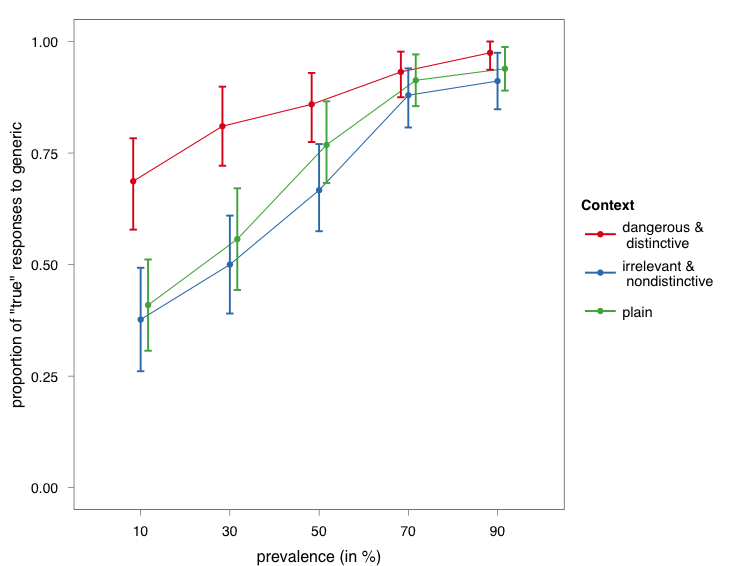
\includegraphics[width=\columnwidth]{data_truthconditions1}
%                \caption{Truth conditions of the generic vary across contexts. Error bars denote bootstrapped 95\% confidence intervals.}
%                \label{fig:datatc}
%        \end{subfigure}%
%        ~ %add desired spacing between images, e. g. ~, \quad, \qquad, \hfill etc.
%          %(or a blank line to force the subfigure onto a new line)
%        \begin{subfigure}[t]{0.42\columnwidth}
%                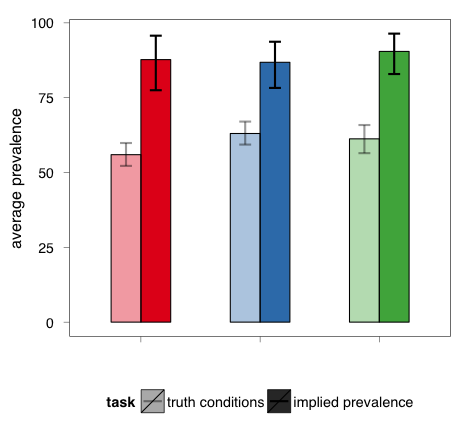
\includegraphics[width=\columnwidth]{data_asymmetry1}
%                \caption{Asymmetry between verification and interpretation, see text for details.}
%                \label{fig:datasym}
%        \end{subfigure}
%        ~ %add desired spacing between images, e. g. ~, \quad, \qquad, \hfill etc.
%          %(or a blank line to force the subfigure onto a new line)
%        \caption{Replication of CBG}\label{fig:exp1}
%\end{figure}

\begin{figure}
\centering
    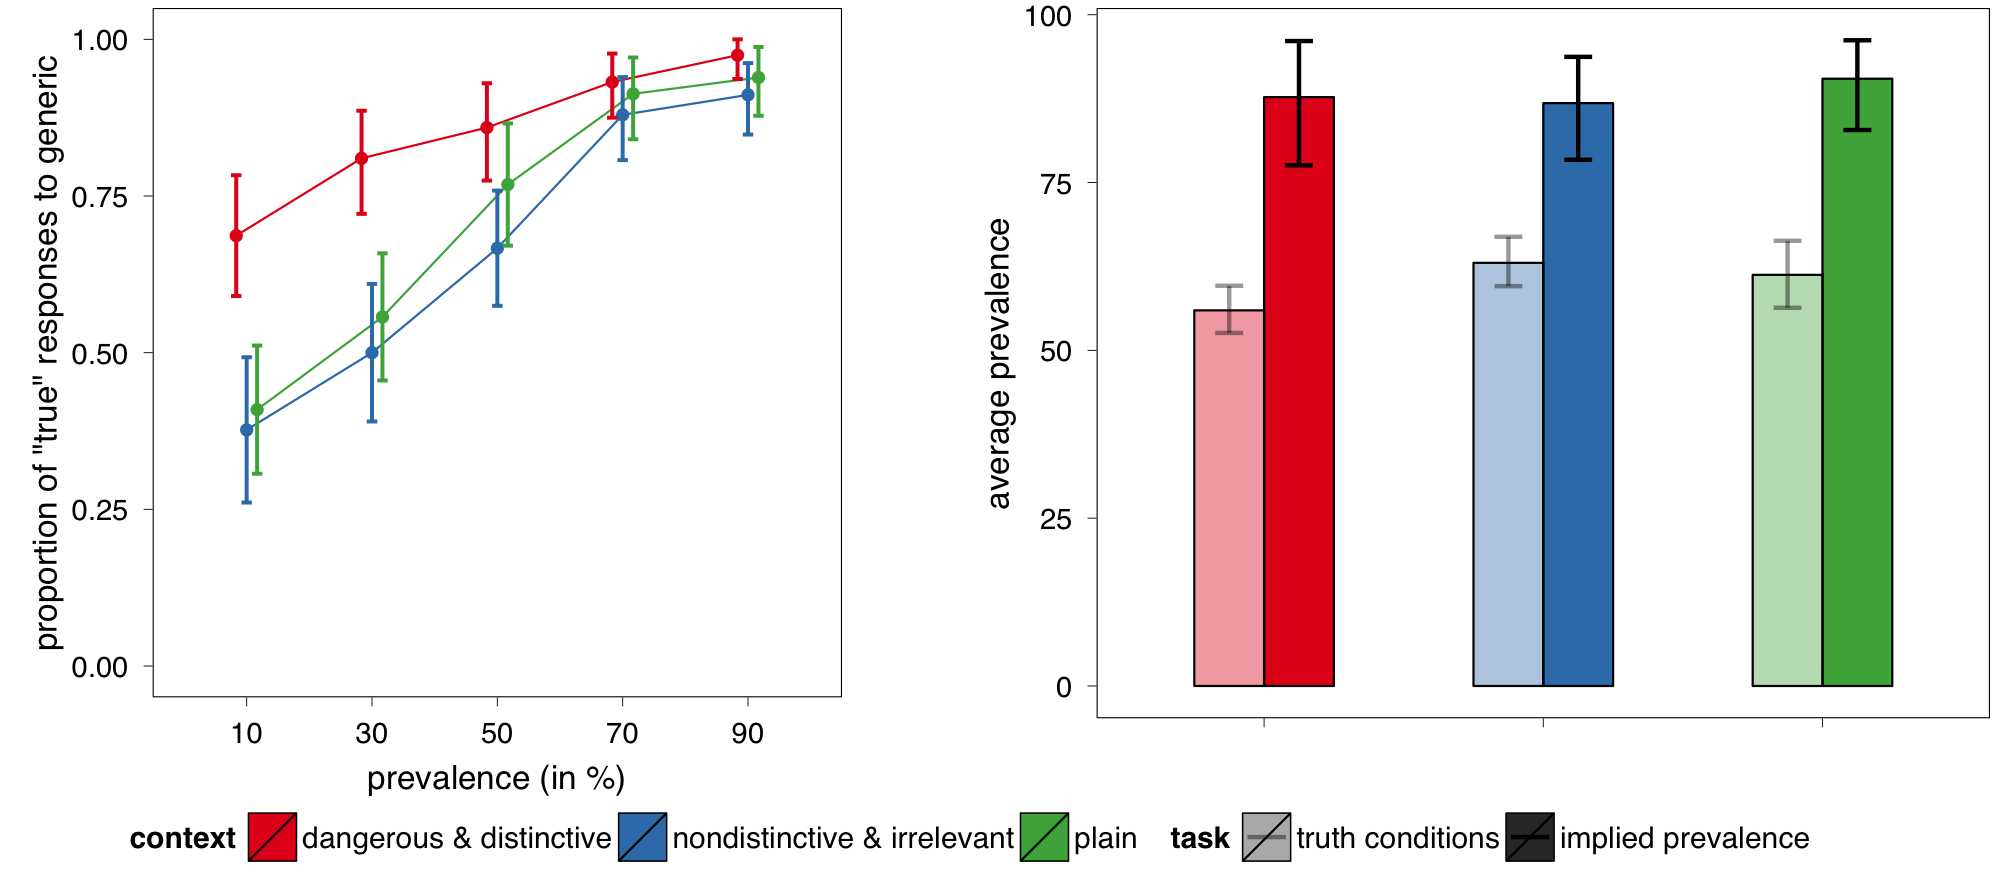
\includegraphics[width=\columnwidth]{Xexp1data}
    \caption{Replication of CBG. Left: \emph{truth conditions} vary by context (Exp. 1a). Right: \emph{implied prevalence} of the generic is greater than \emph{truth conditions} (Exp. 1b).}
  \label{fig:exp1}
\end{figure}

Results are shown in Figure~\ref{fig:exp1} (Left). We entered participants' truth judgments into a mixed effects logistic regression with random by-item and by-participant effects of intercept and fixed effects of prevalence and type as well as their interaction\footnote{This was the maximal mixed-effect structure supported by the data.}.  
%
Our results replicated the finding of CBG that the generic statements were endorsed more with dangerous and distinctive properties than with plain properties (Figure \ref{fig:exp1}, left; $\beta=1.99; SE = .36; z = 5.52; p < .001$). 
%
There was also an interaction between prevalence level and type such that the generic was endorsed more with\emph{DangDist} properties than with plain properties at lower prevalence levels ($\beta=.03; SE = .01; z=2.35; p = 0.019$). There was a trending effect for the \emph{NDangNDist} properties to be endorsed \emph{less} than the plain properties ($\beta=-.57; SE = .30; z=-1.91; p = .056$).

\subsection{Experiment 1b: \emph{implied prevalence}}

\subsubsection{Participants}

We recruited 30 participants over MTurk.  Participants were restricted to those with US IP addresses and with at least a 95\% MTurk work approval rating. All participants were native English speakers. The experiment took about 5 minutes and participants were compensated \$0.50.

\subsubsection{Procedure and materials}

Our procedure was very similar to CBG's \emph{implied prevalence} task. Our instructions were the same as in Exp. 1a\footnote{The experiment in full can be viewed at \url{http://stanford.edu/~mtessler/experiments/generics/cbg2010-replication/experiment/experiment-12.html}}. 

The materials and property-type conditions were the same as in Exp. 1a. Each participant saw 10 trials of each of the 3 property-types (30 trials in total). On each trial, participants saw a generic statement and property-type statements. 
%A context here was either (1) dangerous \& distinct statements (e.g. ``These feathers are as sharp as needles and can easily get lodged in you, causing massive bleeding. No other animals have these kinds of feathers.''), (2) not distinct \& irrelevant statements (e.g. ``These feathers are wide and very smooth to the touch. Other animals have these kinds of feathers.'', or (3) nothing else. 
Participants were then asked ``What percentage of [the kind] do you think have [the property]?'' (e.g. ``What percentage of lorches do you think have purple feathers?'') The dependent measure was a free response required to be an integer, $0-100$. 

\subsubsection{Data analysis and results}
\label{subsec:cbganalysis}

%\begin{figure}
%\centering
%    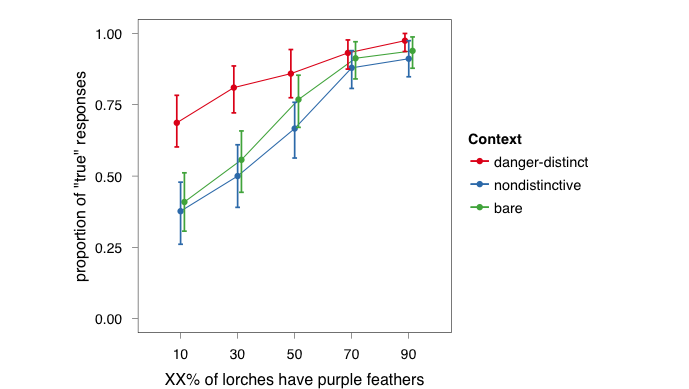
\includegraphics[width=\columnwidth]{fig1_replication}
%    \caption{Replication of CBG \emph{asymmetry}, generics condition}
%  \label{fig:replication}
%\end{figure}
%
To compare the truth conditions data with the implied prevalence data, we followed the data analysis strategy of CBG. Using the data from Exp. 1a, we computed, for each subject, an \emph{average prevalence level} that led to ``True'' responses (e.g. if a participant said ``True'' whenever the prevalence was 70\% or 90\% and ``False'' to everything else, that participant received an \emph{average prevalence score} of 80\%). This score was compared against the implied prevalence dependent measure of Exp. 1b. 

The prevalence scores from each task were entered into a linear mixed model with a by-participant random effect of intercept; the fixed effects were property-type, task, and their interaction. Our results replicated the asymmetry finding of CBG that the generic statement was interpreted as having a higher prevalence than its truth conditions entail (i.e. main effect of task; $\beta=28.8; SE = 4.3; t=6.6; p < 0.001$; see Fig.~\ref{fig:exp1}, right). In the original study, this asymmetry was not observed for sentences using the quantifier ``most''; however, we did not replicate this effect here.

\section{Threshold semantics}
The above results, replicated from CBG, indirectly constrain the effective truth conditions that participants are using for generic statements within these experimental conditions. In this section, we briefly review threshold semantics and the trouble posed by this data.

Let us assume that the conditions for truth of the generic can be usefully represented by a threshold on prevalence: the generic is true when the prevalence of some property within a kind exceeds a given threshold (see \citeA{Cohen1999} for a similar assumption). If we use $x\in [0,1]$ to denote the prevalence $P(\text{property}|\text{category})$, then the simple threshold meaning is:
\begin{align}
 g(x, \theta) = \begin{cases}
   1 & \text{if } x > \theta \\
   0       & \text{if } x \leq \theta
  \end{cases}
%  \tag{\theequation}
   \label{eq:ftsem}
\end{align}
The function $g$ captures a very simple cognitive model in which people evaluate the generic by comparing observed prevalence to the known threshold.
It is apparent that if the threshold $\theta$ were truly fixed, this model could account for neither property-type nor asymmetry effects.

The simplest model that could account for context effects would one in which the threshold was a function of context. 


\subsection{A context-dependent fixed-semantics}

We reexamine our fixed-semantics model, now allowing for the possibility that $\theta$ could vary by property-type: $g(x,\theta_{type})$.

To begin our data analysis, we make no \emph{a priori} assumptions about the (fixed, but unknown to us) values of $\theta_{type}$, placing on it a uniform prior distribution: $\theta_{type} \thicksim U(0,1)$. 
We account for inattention and other irrelevant factors by including a probability $\phi_{task}\thicksim U(0,1)$ for each task that a given response is the result of uniform random guessing\footnote{Ideally, we would have $\phi$ be a function of participant (some participants guess more than others) and experimental condition (some conditions are more difficult or less constrained and invite more guessing). This is computationally too demanding when coupled with the more complex cognitive model explored later.}  \cite{LW2014}.
The inferred ``guessing'' parameter $\phi$ is the amount of data that would have to be attributed to random guessing in order for the fixed-threshold model of the generic to apply to the experimental data. In this sense, $\phi$'s provide a coarse notion of model fit. 

%We attach uniform priors to each of the $\theta_{c}$'s to examine the data from the two experiments. . 

We are now in a position to examine how a truth-functional threshold of the generic would need to behave across these three contexts. 

%\subsubsection{Inferred parameters}

The results can be seen in Figure \ref{fig:justFixed}. 
The posterior distributions for $\phi_{t}$'s show that the amount of data that must be attributed to guessing to be consistent with this model of generics is still quite high: around 45\% for the \emph{truth conditions} task. 
Turning to $\theta_{c}$, there is evidence for the variability of the generic threshold in the \emph{truth conditions} task. In the \emph{plain} context, the analysis suggests the threshold is somewhere between 0\% and 30\%, but it's unclear where exactly in that range the threshold should be. Critically, in the \emph{dangerous and distinctive} context, the analysis infers a lower threshold, less than 10\%. This matches with the earlier Null Hypothesis analysis. Finally, and most intriguingly, the analysis infers a third distinct threshold profile for the \emph{nondistinctive and irrelevant} context.  The inferred threshold is greater than 10\%, but could be as high as 50\%. This is an overall higher inferred threshold for the nondistinctive category; however, these results are inconclusive as to whether or not this threshold is actually different from the \emph{plain} context.



\begin{figure}
\centering
    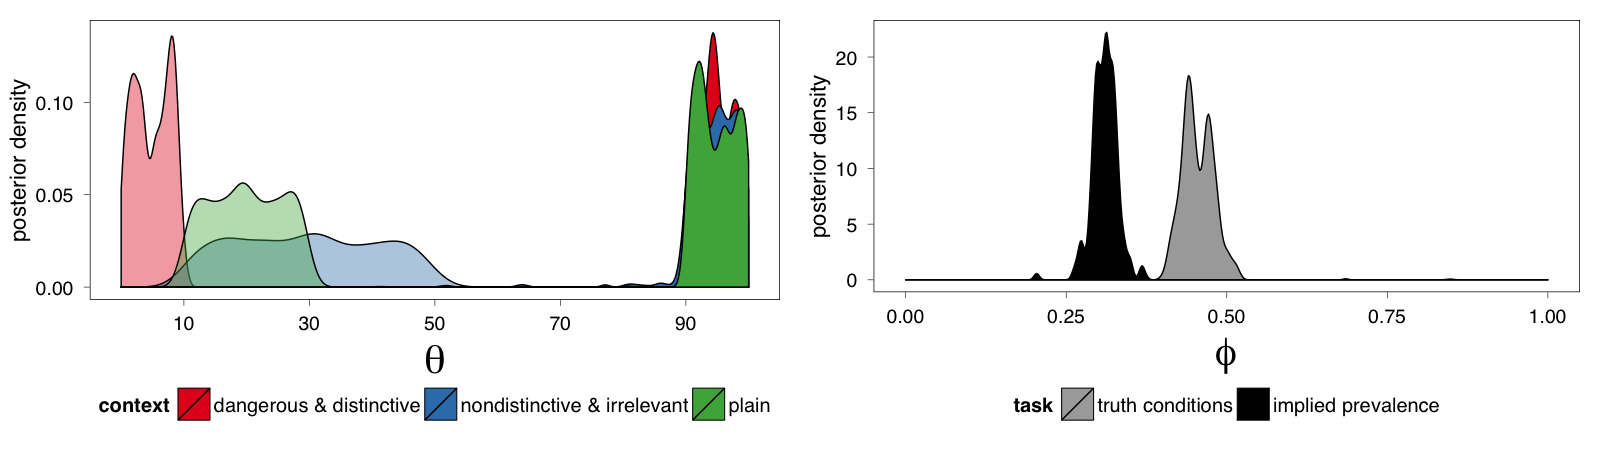
\includegraphics[width=\columnwidth]{fixed_phis_thetas}
    \caption{Analysis of the context-dependent fixed-semantics of a generic. Left: Inferred threshold for each experiment and context. Right: ``guessing'' parameter for each experiment.}
  \label{fig:justFixed}
\end{figure}




%\subsubsection{Posterior predictives}

The fixed-semantics model can also be evaluated by examining the posterior predictive distribution of responses. 
The posterior predictive distribution marginalizes over the inferred parameter values to produce predictions about what the data should look like given the cognitive model and the observed data. This is akin to fitting the parameters and is an important step in model validation as it shows what data is actually predicted by the model.
%\footnote{As a thought experiment, consider 2 coins assumed to come from a single coin-making machine (all the coins from this machine have the same weight). You flip each coin 100 times. The first one returns 100 heads, and the second one returns 100 tails. The posterior mean of the inferred coin weight will be 0.5. Comparing the posterior predictive distribution (based on this inferred coin-weight) to the observed data, however, will highlight the fact that your theory about the ``single coin-making machine'' is seriously flawed.}.
Following directly from the inferred $\theta_{c}$'s, the model matches the ordering of the truth-conditions by context reasonably well. However, the model predicts an abrupt transition in endorsement rates for prevalences on either side of the threshold; the model is too dichotomous to match the human data. The correlation between the posterior predictive and the data is a moderate $r = 0.81$. 

The fixed-threshold semantics model is not flexible enough to explain the observed data, but it has an even more serious flaw: the variation of threshold by condition is postulated \emph{a priori} in the data analysis, rather than accounted for by the cognitive model. That is, participants in our experiment must have some way of arriving at different thresholds for different tasks and conditions, which this model has no means to explain. For a more explanatory model we turn to the pragmatics of language understanding.

%
%
%
%To set the stage for future Bayesian analyses, let us nonetheless explore the quantitative relation of a context-invariant threshold semantics to the data.
%
%\subsection{A context-invariant fixed-semantics}
%%We first examine what this threshold would look like if it were invariant to context and task. 
%To begin our data analysis, we make no \emph{a priori} assumptions about the (fixed, but unknown to us) value of $\theta$, placing on it a uniform prior distribution: $\theta \thicksim U(0,1)$. 
%We account for inattention and other irrelevant factors by including a probability $\phi_{t}\thicksim U(0,1)$ for each task that a given response is the result of uniform random guessing\footnote{Ideally, we would have $\phi$ be a function of participant (some participants guess more than others) and experimental condition (some conditions are more difficult or less constrained and invite more guessing). This is computationally too demanding when coupled with the more complex cognitive model explored later.}  \cite{LW2014}.
%The inferred ``guessing'' parameter $\phi$ is the amount of data that would have to be attributed to random guessing in order for the fixed-threshold model of the generic to apply to the experimental data. In this sense, $\phi$ gives a coarse notion of model fit. 
%%We analyze the data from Exp. 1a and 1b jointly as well as independently.
%
%
%%Following standard practice in Bayesian data analysis \cite{LW2014}, we include the data-analytic parameter $\phi$ to account for data points that deviate strongly from our theory; it is a guessing parameter. We assume there is some proportion of responses where the participant is responding randomly, and we estimate this quantity by way of $\phi$. We model two such $\phi$ parameters, one for each task.
%%
%%\begin{align*}
%%\theta \thicksim U(0,1) \\
%%\phi_{t} \thicksim U(0,1) %\mid  t \in \{exp1a, exp1b\}
%%\end{align*}
%
%
%%We formalize the notion of ``effective truth conditions'' by saying the generic is a function from states of the world to truth-values. We operationalize \emph{states of the world} here as the prevalence of some property within a kind. This mapping is then determined by some threshold such that the generic is true when the prevalence is above threshold. 
%
%%Using the Church probabilistic programming language to represent this model \cite{probmods}, this would be written:
%%
%%\begin{lstlisting}
%%(define generic 
%%	(lambda (prevalence) (> prevalence generic-threshold)))
%%\end{lstlisting}
%
%%To handle the inference problem the participant is faced with, we express the subject's uncertainty about whether the generic is true or false.
%%
%%\red{NDG: the rest of this section is too long and doesn't make sense to me...}
%% \begin{lstlisting}
%%(define truth-conditions (lambda (prevalence)
%%	(query  
%%	
%%		(define generic ...) ;defined as above
%%		(define generic-is-true? (flip 0.5))
%%		
%%		generic-is-true?
%%			
%%		(generic prevalence))))
%%\end{lstlisting}
%
%
%
%%\subsubsection{Inferred parameters}
%
%
%
%A joint analysis of the data from Exp. 1a and 1b, produces the expected extreme results. The inferred $\phi_{1a}$ is near 1, $\phi_{1b}$ has a more reasonable posterior mean of 0.3, and the inferred $\theta$ is near 100\%. That is, the best interpretation of the data discounts the \emph{truth conditions} data entirely and uses only the \emph{implied prevalence} data to set the threshold, which results in interpreting the generic as a universal quantifier.
%A separate by-experiment analysis produces thresholds that are completely different for the two tasks. 
%For the implied prevalence task, the threshold is again close to 100\%. 
%For the truth conditions task, the threshold is probably greater than 10\% and less than 30\%\footnote{This uncertainty results from the sparseness of our measure: participants were queried only at prevalence levels 10, 30, 50, 70, and 90\%.}.
%
%%The amount of guessing for the \emph{truth conditions} task ($\phi_{1a}$) is no longer near 1, but is still quite high, around 0.5, which means that participants would have to be guessing 50\% of the time. Though this analysis shows an asymmetry between the two tasks, it doesn't have the ability to capture the context-dependence present in the data. 
%%we already know there is an effect of context on the generic meaning. There is no way for this model to account for such data.
%
%%\begin{figure}
%%\centering
%%    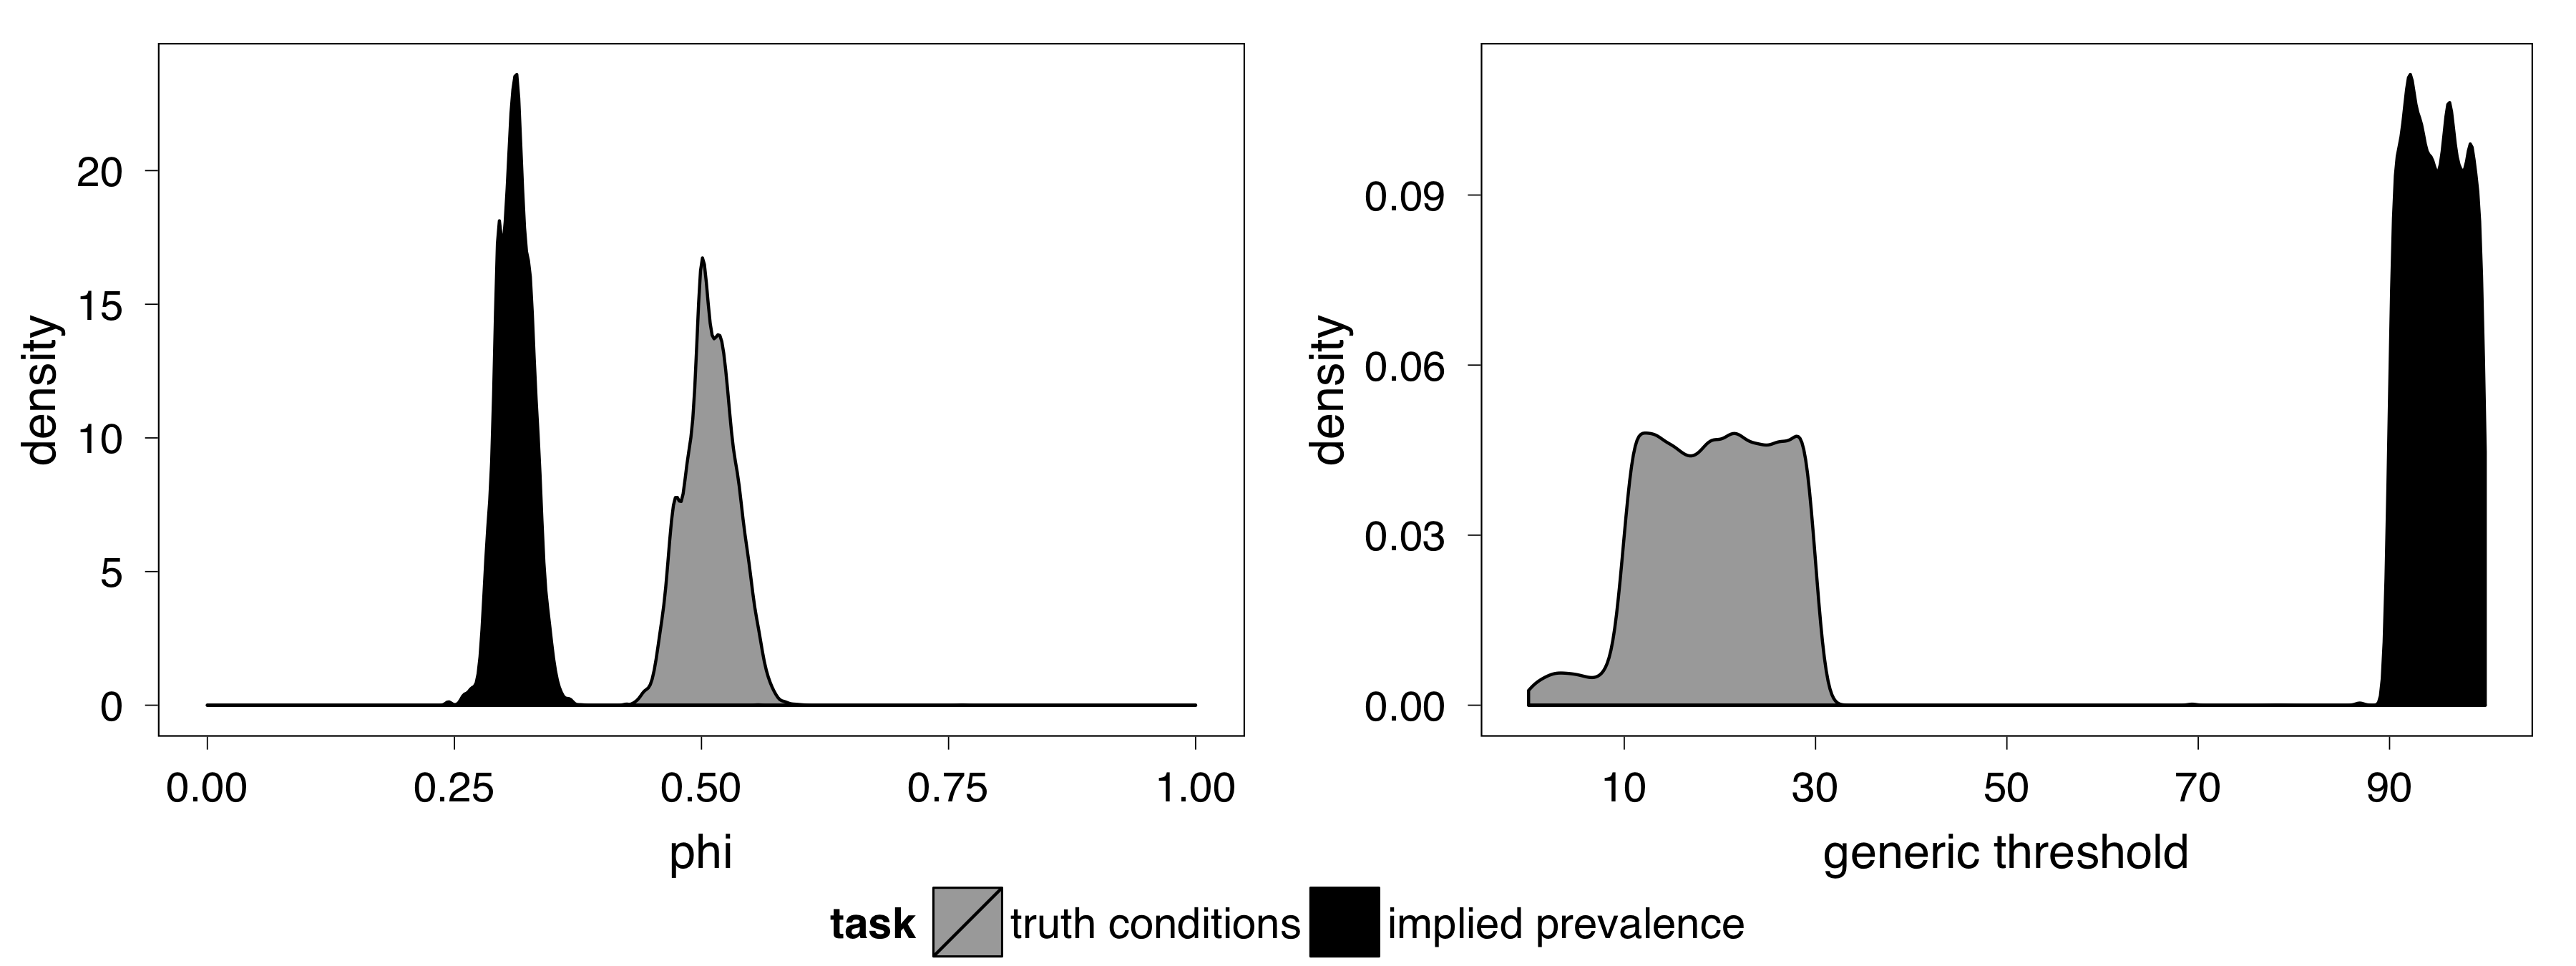
\includegraphics[width=\columnwidth]{trulyFixed_phis_thetas}
%%    \caption{Fixed and context-invariant semantics of a generic. Inferred ``guessing'' parameter (left) and threshold (right) for each experiment.}
%%  \label{fig:trulyfixed}
%%\end{figure}
%
%


\section{Reasoning about the threshold}

%CBG showed how contexts affects the endorsement for generic statements. An additional concern of their experiments surrounded the relation between two dependent measures for understanding generics. One dependent measure was the ``truth conditions'', or \emph{sentence verification} measure that we've been considering up to this point. The other was an ``implied prevalence'', or \emph{sentence interpretation} dependent measure. The latter was collected by giving participants the generic statement (plus, any additional contextual information), and asking the participant ``What percentage of lorches have purple feathers?''

The tasks in Exp.~1 are, fundamentally, language understanding tasks. We draw on recent work from probabilistic pragmatics to formalize our intuitions about how listeners arrive at interpretations of utterances. In particular, we draw on work from the Rational Speech Act (RSA) theory of language understanding. In this framework, a listener infers the meaning of an utterance by considering the thought-processes of a speaker whose goal is to be informative. Variants of this theory have provided computational explanations for a number of linguistic phenomena including scalar implicature, hyperbole, and argument evaluation \cite{Kao2014, Tessler2014, Lassiter2014}. 

%\subsection{Lifted-variable RSA}

%The Bayesian data analysis above provides compelling evidence that context influences the truth-conditions of a generic statement. The poor qualitative fit as well as the high inferred value of the guessing parameter $\phi$ suggest, however, that our language model is incomplete. Rather than propose that the meaning of a generic is simply a one-to-one mapping between context and threshold, 

We propose that the literal semantics of a generic sentence is in fact a threshold on prevalence, but listeners don't know the appropriate threshold and actively reason about it in context. 
A similar proposal has been made to explain gradable adjectives like \emph{tall}. 
\citeA{Lassiter2015}  propose the meaning of an adjective like \emph{tall} is a standard truth-functional meaning such that the object in question \emph{is tall} if it has a height greater than the threshold $\theta_{tall}$. 
The vagueness and context-sensitivity of scalar adjectives are accounted for by treating $\theta_{tall}$ as an unknown property of the language, and modeling the pragmatic listener as inferring this threshold.
 
%The key insight, though, is that the listener has uncertainty about what $\theta_{tall}$ actually is, and infers that value of $\theta_{tall}$ via the same recursive reasoning process through which she infers the intended meaning of the utterance.

%How is a listener supposed to reason about $\theta_{tall}$? In the case of adjectives, reasonable thresholds are inferred by way of the prior distribution of the property in question. ``John is tall'' and the ``Empire State Building is tall'' imply different heights for John and the ESB because the prior distributions of heights for people and buildings are different. An adjective will only be informative (and truthful) with respect to the appropriate prior distribution. 



%In Church, the model looks like:
%
%\begin{lstlisting}
%(define pragmatic-listener (lambda (utterance)
%	(query
%		(define prevalence (prevalence-prior))
%		; listener doesn't know the threshold
%		(define generic-threshold (threshold-prior))
%			
%		prevalence
%			
%		(equal? utterance 
%		; listener imagines the speaker does know the threshold
%			(speaker prevalence generic-threshold)))))
%			
%(define speaker (lambda (prevalence generic-threshold)
%	(query
%		(define utterance (utterance-prior))
%			
%		utterance
%			
%		; speaker conditions on a literal-listener inferring the right prevalence
%		(equal? prevalence 
%			(literal-listener utterance generic-threshold)))))
%			
%(define literal-listener (lambda (utterance generic-threshold)
%	(query
%		(define prevalence (prevalence-prior))
%			
%		prevalence
%		; literal listener conditions on the words being true
%		(utterance prevalence generic-threshold))))
%\end{lstlisting}

The RSA model for generic interpretation, with the prevalence threshold as a variable ``lifted'' to pragmatic reasoning is specified by:
\begin{flalign}
& P_{L_{0}}(x \mid g, \theta) \propto g(x, \theta) P(x) \label{eq:L0} \\
& P_{S_{1}}(g \mid x, \theta) \propto {P_{L_{0}}(x \mid g, \theta)} \label{eq:S1}\\
& P_{L_{1}}(x , \theta \mid g) \propto P_{S_{1}}(g \mid x, \theta) P(x) \label{eq:L1}
\end{flalign}
The literal content of the generic in Eq.~\eqref{eq:L0} is identical to the fixed-threshold model in Eq.~\eqref{eq:ftsem}. However, it interacts with the prior distribution $P(x)$ over prevalence levels---the prior distribution of prevalence of a particular property across kinds.

Eq.~\eqref{eq:L1} is a model of a listener ($L_{1}$) who has been told a generic statement. She assumes that, whatever the speaker ($S_{1}$) meant to communicate, the speaker was trying to be informative and that his goal was to communicate the prevalence $x$. She assumes the speaker in Eq.~\eqref{eq:S1} knows $\theta$ and chooses an utterance to be informative to the literal listener ($L_{0}$).  From this, the listener jointly infers both $x$ and $\theta$. We call this type of model a ``lifted variable'' model (lvRSA) because $\theta$, traditionally thought to be part of the semantic content of the utterance (and thus perfectly transparent to all in the conversation), has been underspecified in the semantics but is locally fixed by pragmatic reasoning.

The prevalence prior $P(x)$ has a critical effect on the interpretation of the generic in this model. As a simplification, we posit a family of possible priors $x \thicksim \beta(\gamma,\delta)$\footnote{For ease of interpretation, we are parametrizing the $\beta$ distribution by its mean and concentration. To recover the canonical shape parametrization, use $\gamma \delta$ and $(1-\gamma)\delta$.}. We hypothesize that the details of this prior (i.e.~$\gamma$ and $\delta$) may differ according to the context in which a generic is used. For instance, when you know that a particular property is rare, a different distribution over categories is called to mind, than if the property is common. This results in different meanings for the generic. Below we infer appropriate prior parameters for each context from the behavioral data.

Following the advice of \citeA{Degen2014}, who investigated the relationship between dependent measures and speaker and listener roles in RSA, we will model the \emph{implied prevalence} task as a pragmatic listener ($L_{1}$) task, but the \emph{truth conditions} task as a pragmatic speaker task. We model the truth judgment with a speaker $S_{2}$ who is trying to convey the prevalence to a pragmatic listener, but can only produce the generic or its negation (i.e.~yes or no to the truth of the generic):
\begin{equation} 
P_{S_{2}}(g \mid x) \propto {P_{L_{1}}(x \mid g)}.
\label{eq:S2}
\end{equation}
The speaker in \eqref{eq:S2}, like $L_{1}$, doesn't know the threshold, but knows that $L_{1}$ is thinking about it, and marginalizes over possible values: $ P_{L_{1}}(x \mid g) = \sum_{\theta} P_{L_{1}}(x , \theta \mid g) $.


%\begin{lstlisting}
%(define lifted-speaker (lambda (prevalence)
%	(query
%		(define utterance (utterance-prior))
%			
%		utterance
%			
%		(equal? prevalence (pragmatic-listener utterance)))))	
%\end{lstlisting}


%\subsection{Bayesian analysis to infer priors}


%\begin{lstlisting}
%(define bayesian-data-analysis
%	(query
%	
%		(define gamma ; mean prevalence
%			(lambda (context) (uniform 0 1)))
%			
%		(define delta ; concentration of our distribution around the mean
%			(lambda (context) (uniform 0 5)))
%			
%		(define phi (uniform 0 1)) ; guessing parameter
%	
%		(define lifted-speaker ...) ; lvRSA model
%		(define pragmatic-listener ...)
%		(define speaker ...)
%		(define literal-listener ...)
%				
%		'(gamma delta)
%				
%		(and 
%			(= experiment1a-data lifted-speaker)
%			(= experiment1b-data pragmatic-listener))))
%\end{lstlisting}

%\begin{figure}
%\centering
%    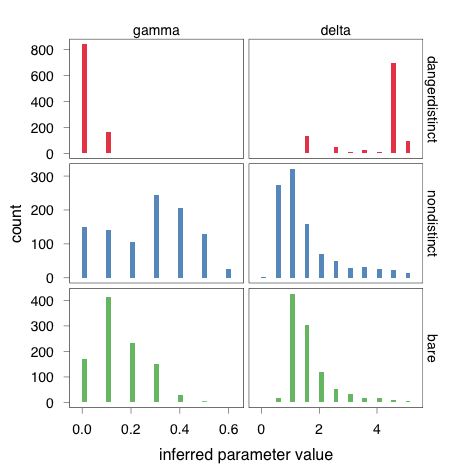
\includegraphics[width=\columnwidth]{fig4_bda2_hyper}
%    \caption{Hyperprior parameters for lifted-variable RSA model}
%  \label{fig:bda2hyperparams}
%\end{figure}

\subsection{Results}

To evaluate this model we perform a Bayesian data analysis similar to that used above.
%to evaluate this more sophisticated cognitive model. We are interested in how the hyperprior parameters $\gamma$ and $\delta$ might vary across contexts.
We infer the parameters of the prevalence prior, $\beta(\gamma,\delta)$, outside of the lvRSA cognitive model (but inside of the data analysis model), using uninformative priors:
$\gamma_{c} \thicksim U(0,1)$,  $\delta_{c} \thicksim U(0,5)$, $\phi_{t} \thicksim U(0,1)$,
%\begin{align*}
%\gamma_{c} \thicksim U(0,1) \\
%\delta_{c} \thicksim U(0,5) \\
%\phi_{t} \thicksim U(0,1) 
%\end{align*}
where $c \in \{DD,NI,P\}$ and $t \in \{$truth conditions, implied prevalence$\}$.
We keep the data-analytic guessing parameters $\phi_{t}$ as a gross estimate of the proportion of responses not captured by our model of cognition. 



%We propose that, in this paradigm, nobody knows $\theta$.  $\theta$ is influenced by the prior distribution over prevalence, which in turn is influenced by the contextual information provided (\emph{DD}, \emph{NI}, or \emph{P}). This contextual information could imply different $P(x)$, prior probability distributions over the prevalence of a property. 
%
%Naively, this distribution would be $U(0,1)$, or equivalently, $\beta(1,1)$. However, we propose that people have different prior distributions in mind, depending on features of the properties under discussion (e.g. distinctiveness).
%
%Although we might have some intuitions what these prior distributions might look like, we put uncertainty over the parameters of this Beta distribution $\beta(\gamma,\delta)$, outside of the RSA model but inside of the data analysis model. 
%
%\begin{align*}
%x_{c} \thicksim \beta(\gamma_{c},\delta_{c}) \\
%\gamma_{c} \thicksim U(0,1) \\
%\delta_{c} \thicksim U(0,5) \\
%\phi_{t} \thicksim U(0,1) 
%\end{align*}
%
%Here, $c \in \{DD,NI,P\}$ and $t \in \{$truth conditions, implied prevalence$\}$.
%
%Thus, we do Bayesian data analysis on a Bayesian Rational Speech-Act model of language understanding, to see how context might influence the prior distribution given the data we've observed. We keep the data-analytic guessing parameters $\phi_{t}$ as a gross estimate of the proportion of responses our model of cognition doesn't capture. 
\begin{wrapfigure}{l}{0.5\columnwidth}
\vspace{-16pt}
  \begin{center}
    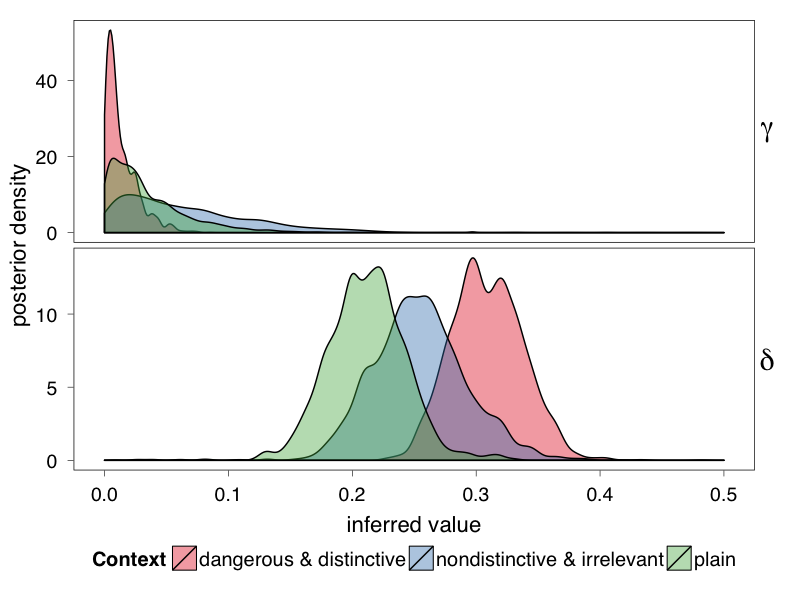
\includegraphics[width=0.48\columnwidth]{inferred_hyperpriors}
  \end{center}
  \caption{Posterior distributions of the hyperprior parameters used in lvRSA.}
   \label{fig:posthyper}
\end{wrapfigure}


%\begin{wrapfigure}{l}{0.5\columnwidth}
%  \begin{center}
%    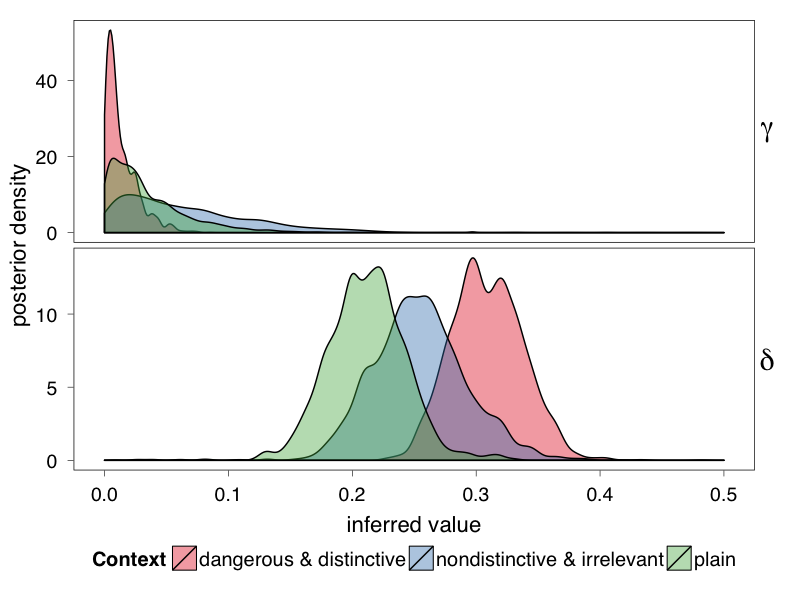
\includegraphics[width=0.48\columnwidth]{inferred_hyperpriors}
%  \end{center}
%  \caption{Posterior distributions of the hyperprior parameters used in lvRSA.}
%   \label{fig:posthyper}
%\end{wrapfigure}


%\begin{figure}
%\centering
%    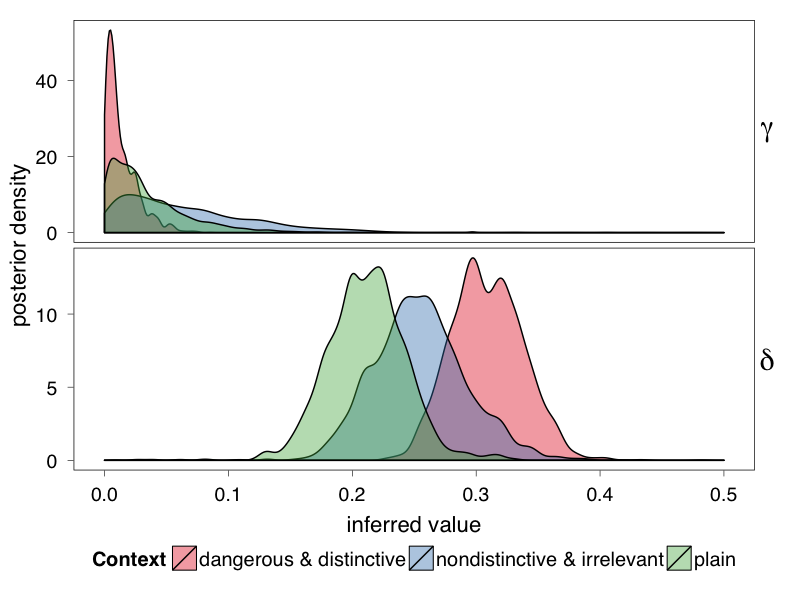
\includegraphics[width=\columnwidth]{inferred_hyperpriors}
%  \caption{Posterior distributions of the hyperprior parameters used in lvRSA.}
%   \label{fig:posthyper}
%\end{figure}

\subsubsection{Inferred parameters}
The mean inferred values of  $\phi_{1a}$ and $\phi_{1b}$ are about 0.08 and 0.05, respectively, a reasonable rate of ``guessing'' for participants on Amazon's Mechanical Turk, indicating that this cognitive model is doing a much better job of accounting for the signal in participants' responses.

%We use Bayesian data analysis to infer the values of the hyperprior parameters $\gamma$ and $\delta$ for the Bayesian lvRSA model. 



Figure \ref{fig:posthyper} shows the posterior distributions of the hyperprior parameters, $\gamma$ and $\delta$, for the lvRSA model. The posterior means for the $\gamma$'s are well-ordered: $DD < P < NI$. This can be directly interpreted as the mean prior prevalence for the three contexts: \emph{dangerous and distinctive} properties are more rare than the other two types of properties. 
The $\delta$'s are much lower than 1 in each case, indicating bi-modal priors peaked at 0 and 1.
The posterior means for the $\delta$'s are also ordered, suggesting that participants may treat variance of prevalence as higher in the \emph{DD} context (or simply be more confused).




%\begin{wrapfigure}{r}{0.5\textwidth}
%%\centering
%   \begin{center}
%    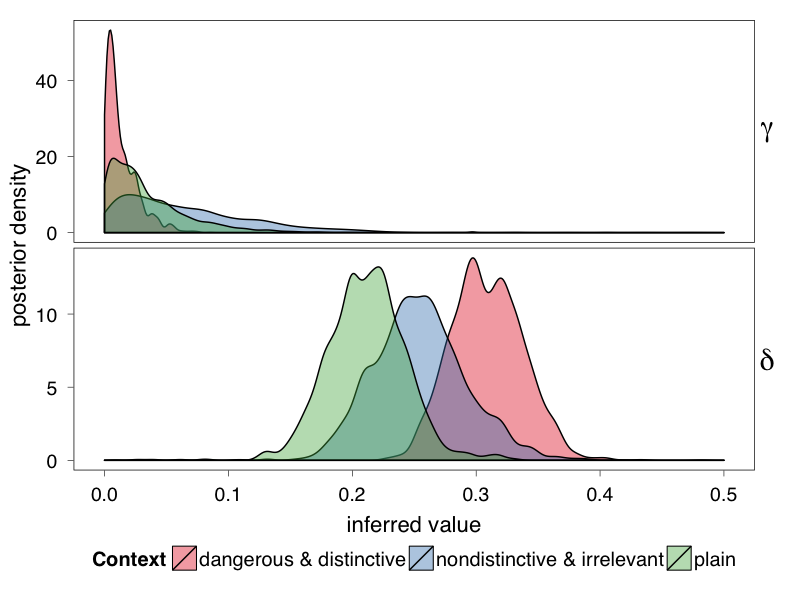
\includegraphics[width=0.48\columnwidth]{inferred_hyperpriors}
%    \end{center}
%    \caption{Posterior distributions of the hyperprior parameters used in lvRSA.}
%  \label{fig:posthyper}
%\end{wrapfigure}

%begin{table}[h]
%\centering
%\begin{tabular}{c | c | c}
%context / parameter & $\gamma$ & $\delta$ \\
%\hline
%DD                  & 0.016  & 0.321  \\
%NI                  & 0.054  & 0.245  \\
%P                   & 0.031  & 0.204 
%\end{tabular}
%\caption{Posterior means for hyperprior parameters.}
%\label{table:postmeans}
%\end{table}
%

For further visualization, we marginalize over the posterior parameter values to reconstruct a canonical prior distribution over prevalence for each context. Figure \ref{fig:inferredpriors} shows these prior distributions inferred from Exp. 1a \& 1b data via the lvRSA model. 
Qualitatively, they are each bi-modal and the \emph{DD} prior has a lower mean.

\subsubsection{Posterior predictives}

The posterior predictions by lvRSA for the \emph{truth conditions} task are shown in Figure \ref{fig:lvRSAposteriorpred}. 
We can see that the model predicts graded endorsement rates for the generic as a function of prevalence---the model has some persistent uncertainty about the true value of the threshold. This same uncertainty is evident in the curves of Exp. 1a.
With the inferred parameter values of the prevalence prior, the model also matches the differences in endorsement rates between context conditions.
We reconstruct the curves of Figure \ref{fig:exp1} reasonably well; the model--data correlation is $r = 0.90$.

%lvRSA models the \emph{truth conditions} task as a speaker---$S_{2}$ using Eq.~\eqref{eq:S2}---faced with the task of saying whether or not the generic applies to a given prevalence of a property. This utterance is intended for a pragmatic listener---$L_{1}$ using Eq.~\eqref{eq:L1}---who will try to reconstruct the prevalence that $S_{2}$ has observed. Here, we have modeled the \emph{implied prevalence} task as this listener, $L_{1}$, given the utterance, tasked with reconstructing the prevalence. 

We use a similar data analysis strategy as we did for Exp. 1b to compare ``average prevalence'' between verification and interpretation. For the \emph{truth conditions} task, we used the model's posterior probability of saying ``true'' at each prevalence level to simulate trials of the experiment as Bernoulli trials. We simulated 30 trials for each of 1000 imaginary subjects in this way. We then followed CBG's data analysis strategy (as recapitulated in Exp.~1b). The model gives a posterior distribution over prevalences, whose expectation we used to model the \emph{implied prevalence} task. We find the model predicts the asymmetry between interpretation and verification of the generic (see Figure \ref{fig:lvRSAposteriorpred}, right).

%\subsubsection{Discussion}

\begin{figure}
\centering
    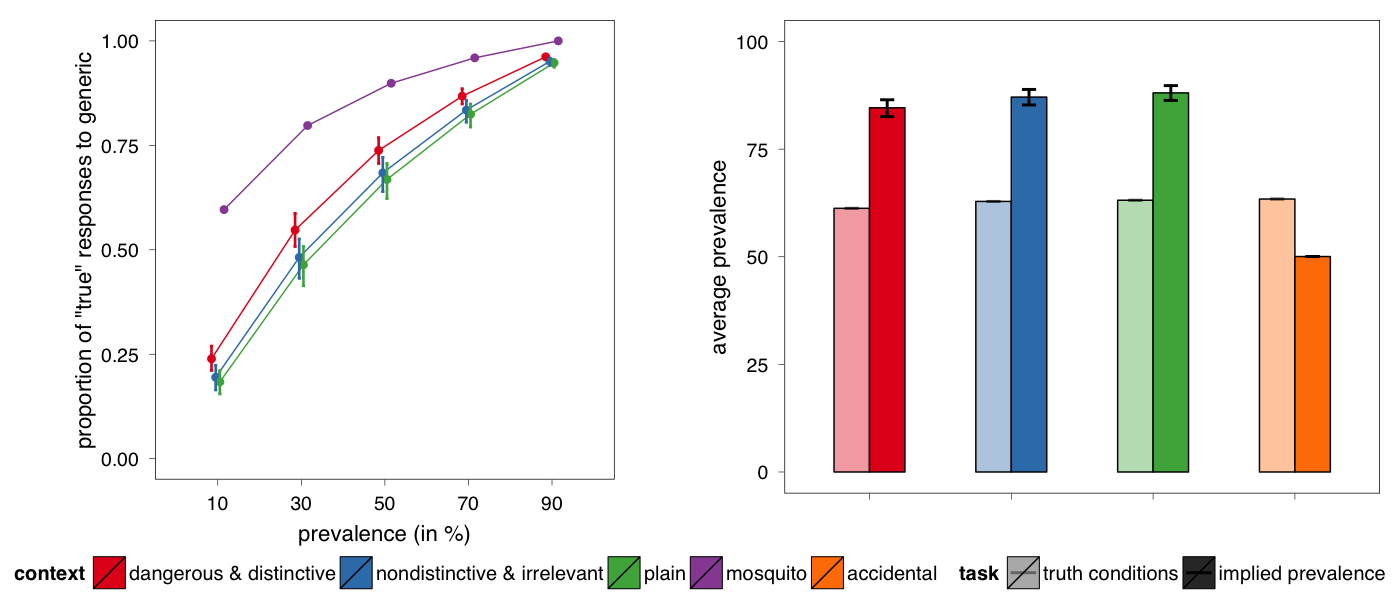
\includegraphics[width=\columnwidth]{lvRSA_postpreds_wSims}
    \caption{Posterior predictives of lvRSA for truth conditions (left) and asymmetry between dependent measures (right). Mosquitos and Accidental predictions use schematic priors (see description in Discussion).}
  \label{fig:lvRSAposteriorpred}
\end{figure}


To see how this asymmetry is possible, consider again the inferred prevalence priors in Figure \ref{fig:inferredpriors}. They are bimodal with peaks around 0\% and 100\%. This is consistent with the intuition that biological properties, such as the ones used by CBG, are properties either held by all of a category or none of a category. Since the semantics of the generic is underspecified (i.e. $\theta$---the threshold of endorsement for truth judgement---is unknown), if $\theta$ falls anywhere in the range between 10\%-90\%, the most likely prevalence is going to be near 100\%. Hence, in the \emph{implied prevalence task}, the most likely inferred prevalence could be appreciably higher than one would expect from the \emph{truth conditions} task. 




%\begin{figure}
%\centering
%    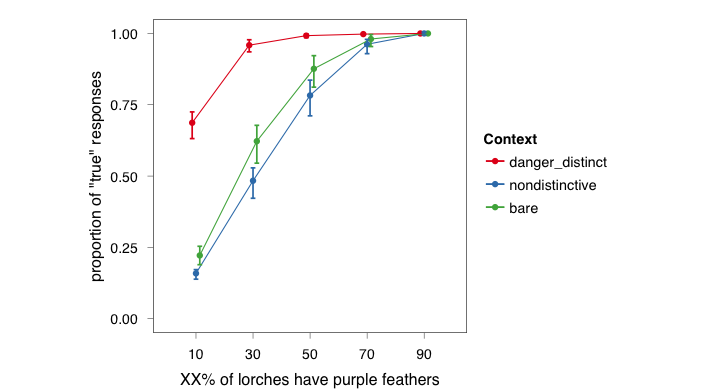
\includegraphics[width=\columnwidth]{fig5_bda2_postpred}
%    \caption{Posterior predictive using lifted-variable RSA}
%  \label{fig:postpred2}
%\end{figure}

Often in Bayesian data analysis, the posterior distribution over parameters is hard to interpret in terms of observable phenomena. Our case is more transparent: if lvRSA were the correct model in this task, the prior distributions of prevalence for the three contexts should look like they do in Figure \ref{fig:inferredpriors}. 
In particular, all three types of properties should have bimodal prior prevalence distributions, with a high probability that 0\% of the kind have the property. Further, this left skew should be more pronounced for the \emph{DD} properties relative to the \emph{P} properties. 

\section{Experiment 2}

\begin{figure}
        \centering
        \begin{subfigure}[b]{\columnwidth}
    			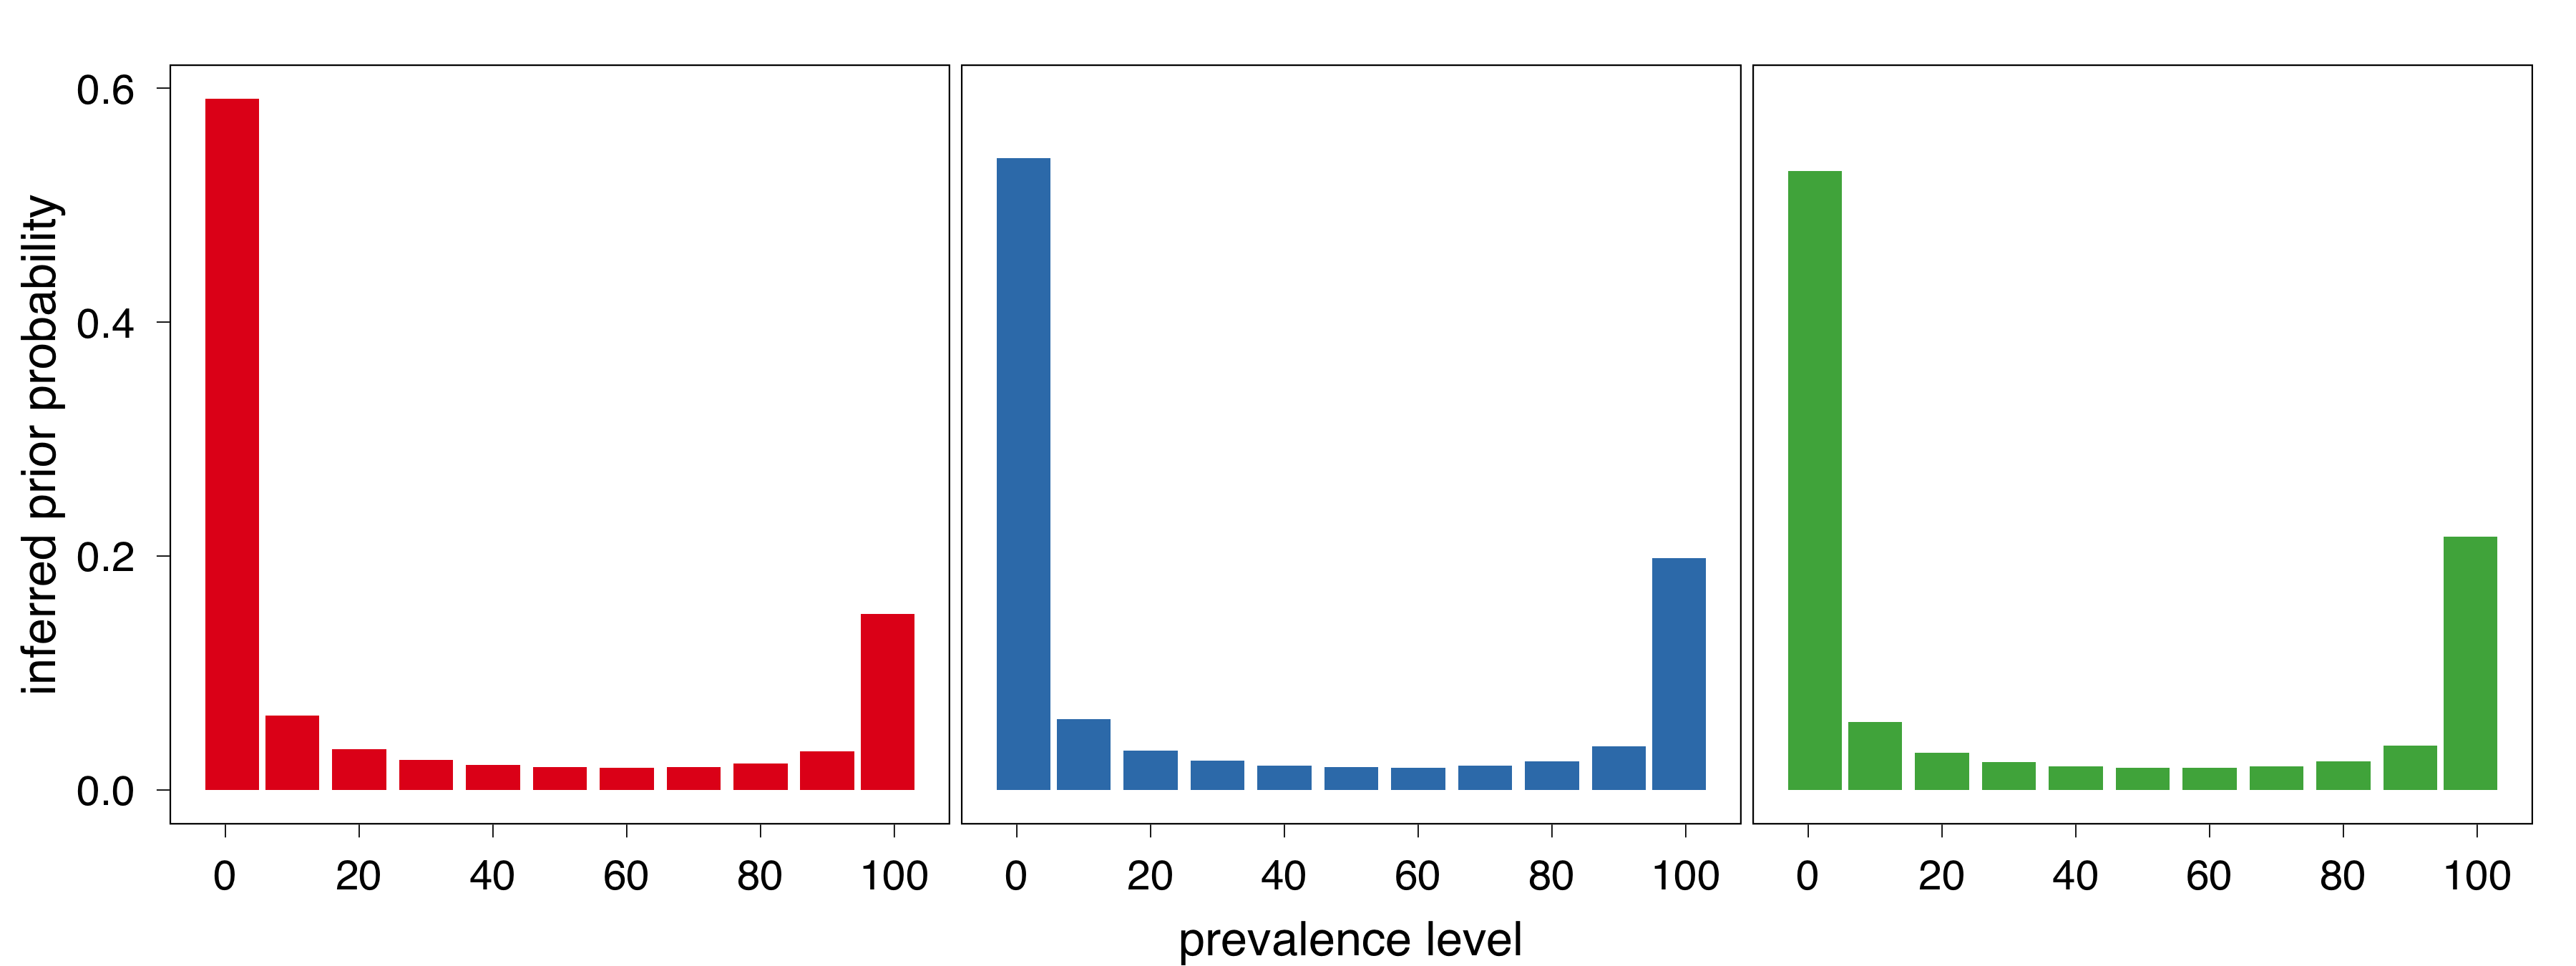
\includegraphics[width=\columnwidth]{inferred_marginalized_priors}
                \caption{Reconstructed priors from marginalized posterior $\gamma$ and $\delta$, for each context.}
                \label{fig:inferredpriors}
        \end{subfigure}%
        
        %add desired spacing between images, e. g. ~, \quad, \qquad, \hfill etc.
          %(or a blank line to force the subfigure onto a new line)
        
        \begin{subfigure}[b]{\columnwidth}
                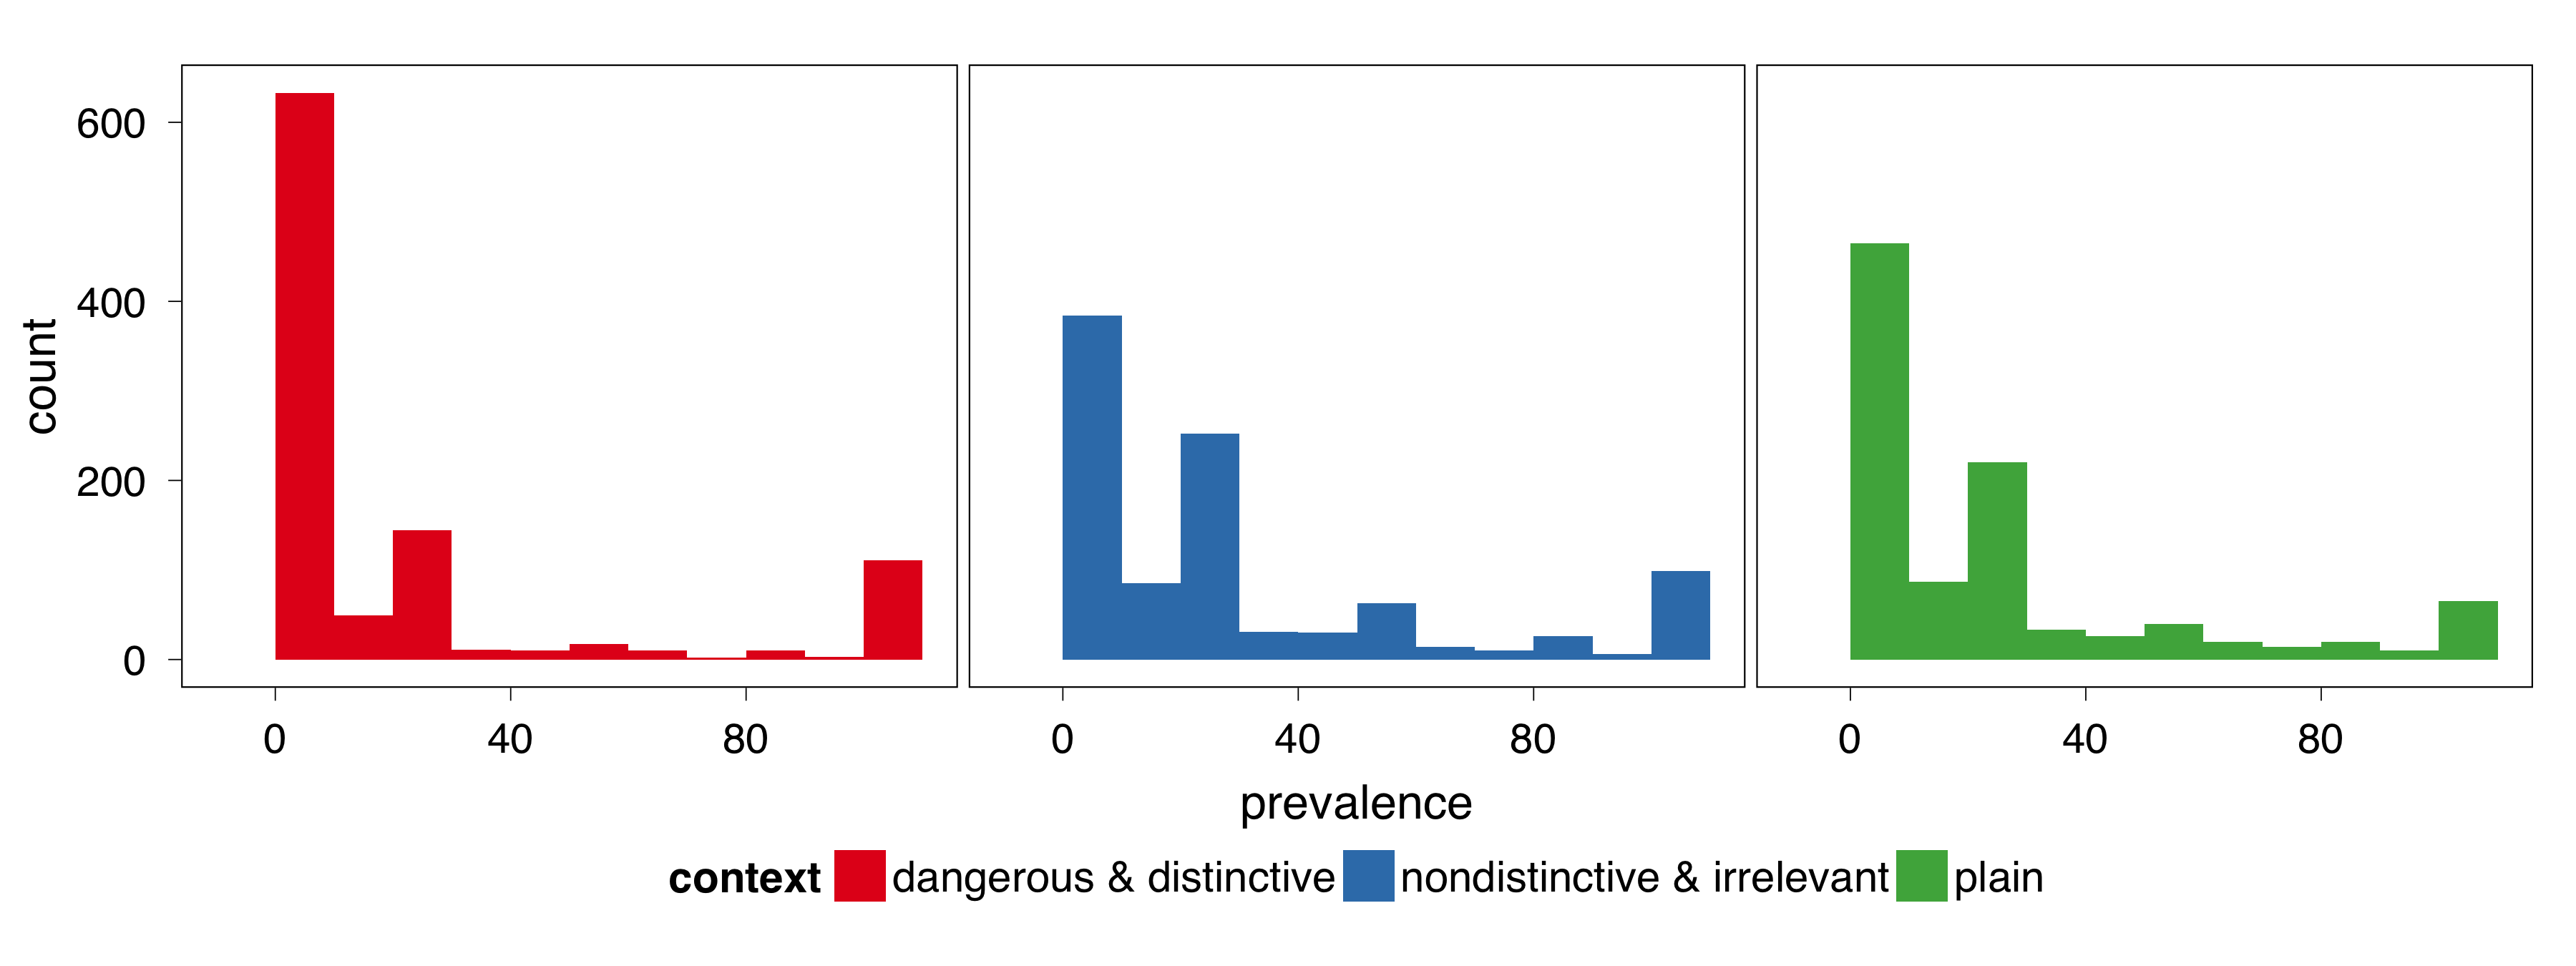
\includegraphics[width=\columnwidth]{elicited_priors}
                \caption{Priors elicited in Experiment 2.}
                \label{fig:elicitedpriors}
        \end{subfigure}
        %add desired spacing between images, e. g. ~, \quad, \qquad, \hfill etc.
          %(or a blank line to force the subfigure onto a new line)
        \caption{Prior distributions over prevalence.}\label{fig:priors}
\end{figure}


Exp. 2 sought to test the prediction that the prior distribution of prevalence levels would be bimodal and vary by context.

\subsection{Method}

\subsubsection{Participants}

We recruited 100 participants over Amazon's crowd-sourcing platform Mechanical Turk. 

\subsubsection{Procedure and materials}

Our procedure\footnote{The experiment in full can be viewed at \url{http://stanford.edu/~mtessler/experiments/generics/cbg2010-replication/experiment/experiment-11.html}} was similar to Exp. 1b. On each trial, participants either read contextual information (\emph{DD} or \emph{NI}) or nothing (\emph{plain}). 

In addition to the contextual information, participants were presented with the following: ``Listed below are 5 kinds of animals, recently discovered.'' and asked the following question: ``What percentage of each kind of animal do you think has [property]?'' The experiment consisted of 6 trials, 2 from each context. 

\subsubsection{Results}

Experiment 2 recovered the shape of the inferred prior distributions predicted from the Bayesian analysis of the lvRSA model (compare Figure \ref{fig:elicitedpriors} to Figure \ref{fig:inferredpriors}). 
%
Hartigans' Dip Test for Unimodality was highly significant for each of the prior distributions ($D = 0.054, 0.084, 0.0745$ for contexts $DD$, $NI$, $P$, respectively; p $<$ 0.0001 for each), and thus the distributions are at least bimodal. 
%
The means of these three distributions are distinct and ordered as predicted (bootstrapped 95\% confidence intervals in parentheses): $\mu_{DD} = 18.1\% (16.0, 20.2), \mu_{P} = 20.8\% (19.0, 22.5), \mu_{NI} = 25.7\% (23.7, 27.6)$.
%
The medians of these three distributions were all significantly different from one another, evidenced by pair-wise Mann-Whitney U tests ($DD$ vs. $P$: $W=417452$; $DD$ vs. $NI$: $W=376180.5$; $NI$ vs. $P$: $W=548994.5$; all $p < 0.00001$). 
%
Finally, the distributions themselves were all significantly different from one another, by Kolmogorov-Smirnov tests ($DD$ vs. $P$: $D = 0.185$; $DD$ vs. $NI$: $D = 0.253$; $NI$ vs. $P$: $D = 0.091$; all $p < 0.001$). In sum, the elicited prior distributions are all at least bimodal, have different central tendencies, and are all distinct.


\section{Discussion}



We have demonstrated the viability of a scalar semantics for generics when coupled with a sophisticated pragmatics. 
A lower-bound threshold on prevalence---the probability of the property given the category---is inferred as part of pragmatic interpretation, yielding vague and context sensitive meanings. 
%We first used Bayesian data analysis to show that the effective threshold of a fixed-threshold semantics would need to vary by context, and yet it still not account adequately for the data. 
%

%
We formalized reasoning about the threshold in a lifted-variable Rational Speech Acts (lvRSA) model. This model predicted graded truth judgements and an asymmetry between truth and prevalence judgements. It also accommodated the role of context, explaining these effects as the result of variation in the prevalence prior. 
In Experiment 2, we verified that participants' beliefs about the prior on prevalence varied in this way. 
This provides evidence that the model we propose can account for many of the empirical phenomena associated with generics.

%We have shown how a Bayesian model of language understanding, motivated by contextual variation of the effective threshold of the generic statement, can explain the puzzling truth conditions and asymmetrical meanings of generic language. We have used techniques in Bayesian data analysis to help arbitrate between two cognitive theories. The first was a simple theory that proposed that a generic was akin to some alien quantifier. In this theory, the generic behaves like other quantifiers in that it has a fixed-threshold semantics. We explored one elaboration of this in allowing the generic to have a threshold that differed across contexts. 
%
%The alternative theory is that there is no generic threshold out there in the world to observe. Instead, listeners infer the threshold (and thus, the semantic content) of the words from context. The posterior predictive distributions of the lvRSA model account for the contextual variation in the generic endorsements, both quantitatively and qualitiative. It further accounts for the asymmetry between verification and interpretation by considering different Questions Under Discussion (QUDs) and communicative roles (speaker / listener) in the two tasks. Finally, the Bayesian analytic techniques allowed us to make a new prediction as to the shape of the prior distribution over prevalence levels for different contexts. Exp. 2 found confirmatory evidence that this is indeed how people think these properties are distributed.

%\section{Further simulations}
%
%Our model makes the prediction that if the shape of the prior distribution was not bimodal, the asymmetry between verification and interpretation would change. Indeed, this is a similar prediction to \citeA{Cimpian2010}, who posited that accidental or disease states (e.g. ``muddy feathers'', ``infected ears'') would weaken the asymmetry. We would expect accidental or disease states to not follow a bimodal distribution. 
 
This model of generic interpretation makes further predictions for situations with qualitatively different prevalence priors. For example, if the prior distribution was unimodal, as in the case with incidental properties (e.g. broken legs), then the asymmetry between verification and interpretation could be dramatically reduced, cease altogether, or reverse (see Figure \ref{fig:lvRSAposteriorpred} for a prediction using the schematic prior in Figure \ref{fig:schematic}). 
Indeed, CBG explored this possibility in one of their experiments using ``accidental and disease states''; consistent with lvRSA, they found no asymmetry. 
Another example is a bimodal prior with a second peak at some low prevalence level (as opposed to a bimodal prior with a second peak at a high prevalence level, which we've focused on in this paper). 
\begin{wrapfigure}{r}{0.5\columnwidth}
  \begin{center}
    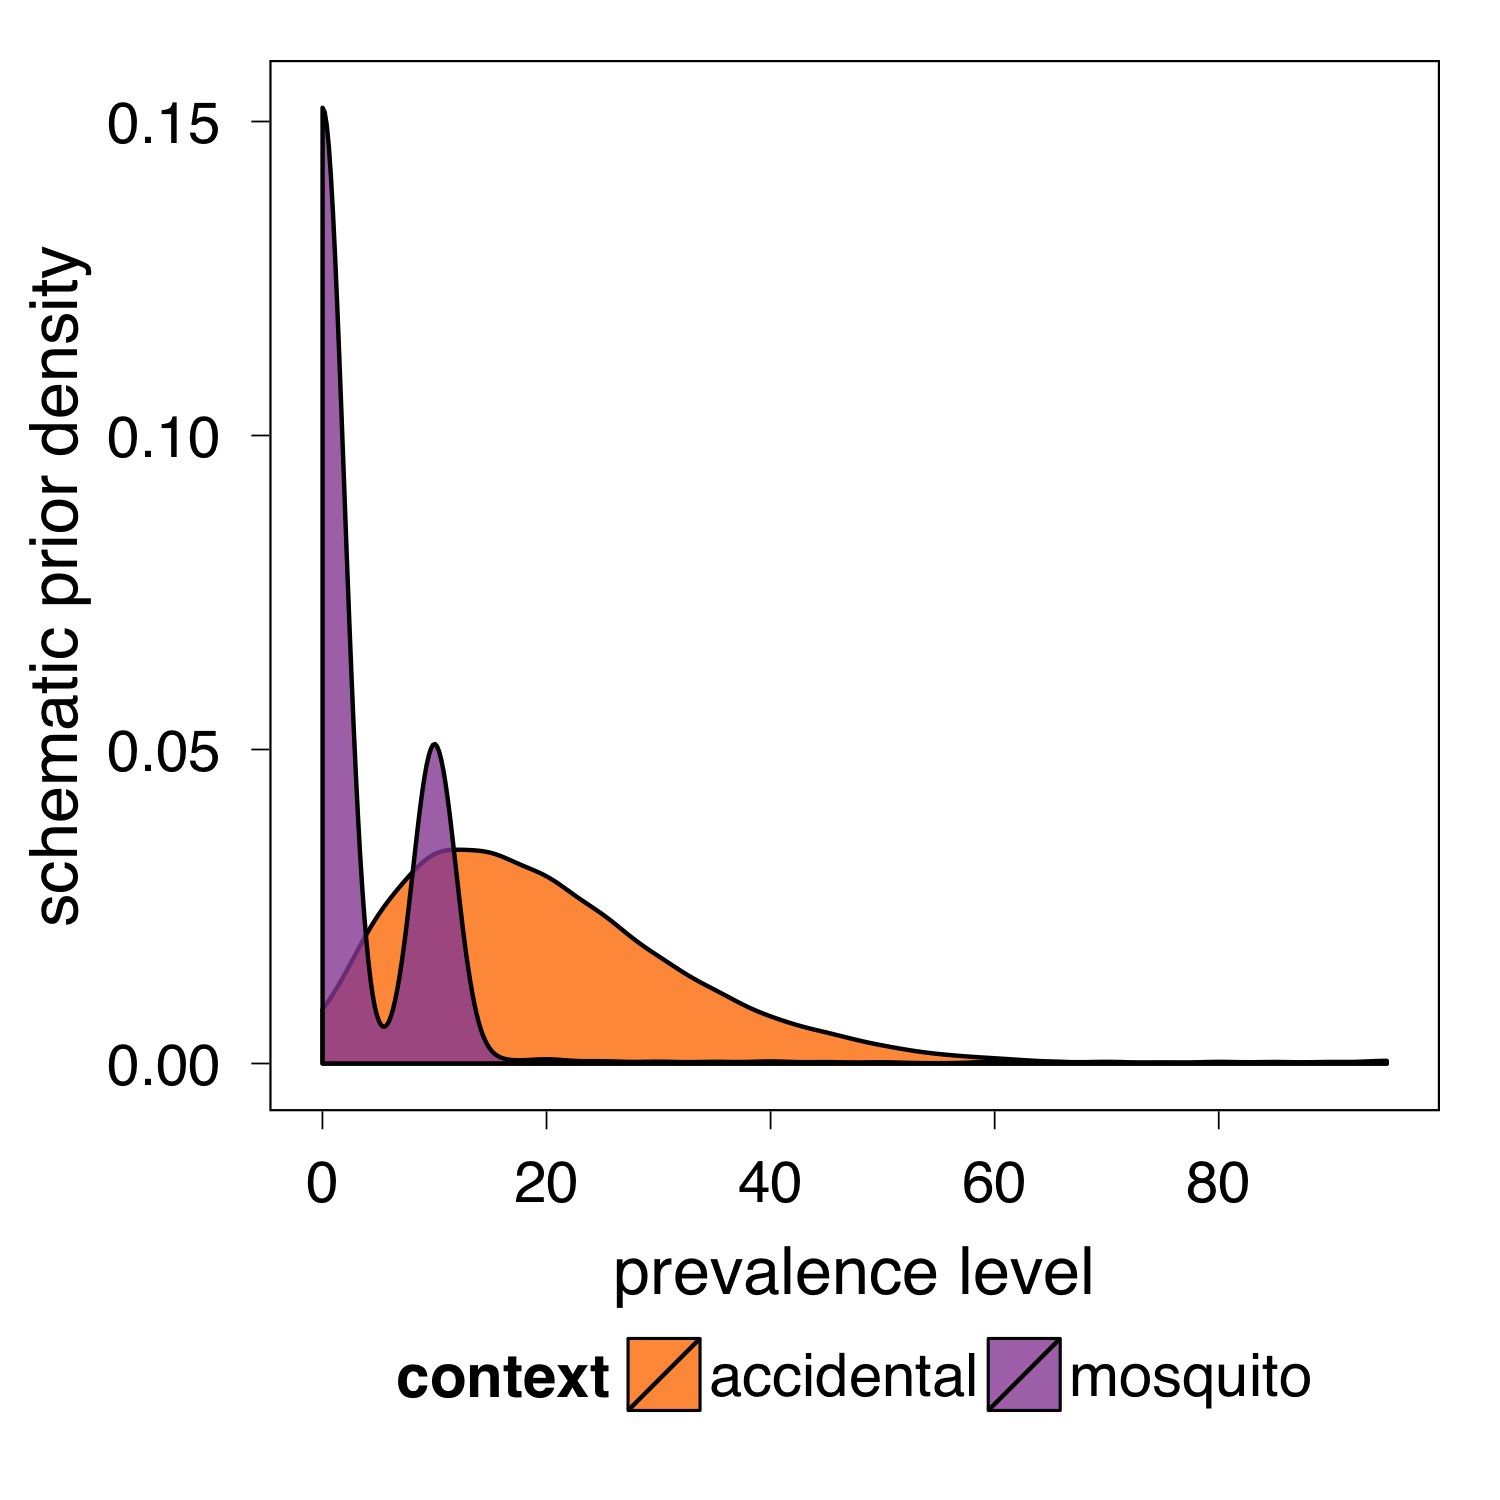
\includegraphics[width=0.48\columnwidth]{schematic_priors}
  \end{center}
  \caption{Schematic priors over prevalence of accidental properties and ``mosquitos with West Nile Virus''.}
   \label{fig:schematic}
\end{wrapfigure}
This prior should describe rare properties that are not only rare \emph{across kinds} but also rare \emph{within kinds}. 
%
%
A canonical example of this is ``West Nile Virus'' in the generic ``Mosquitos carry West Nile Virus''. For a prior like this, the truth conditions for the generic would be relaxed at low prevalence levels, relative to the more common all-or-none priors. We see this behavior using a schematic prior (see Figure \ref{fig:lvRSAposteriorpred} for the truth conditions of the mosquito prior shown in Figure \ref{fig:schematic}). 

Generics are ubiquitous in natural language. It might seem paradoxical, then, that the semantics of generic statements are underspecified. Why should vague language get so much usage? One possibility is apparent in the lvRSA model: generic language provides interlocutors with the flexibility to convey rich meanings, which are easily understood in context. 
Generics are vague, but behaved and useful.

%In this paper, we used techniques of both Bayesian Cognitive Science and Bayesian Data Analysis. The former helped us develop a rich, formal theory of language understanding. These sorts of theories have implications for psychology and linguistics. The latter helped us make inferences about our theories. Bayesian Data Analysis is crucial to make assumptions explicit (e.g. about fixed-threshold semantics) and clean up our data (e.g. discounting behavior that can conceivably be attributed to guessing). Together, they embody a manifestation of a more general philosophy of science: making assumptions explicit and beginning our science by announcing our uncertainty.


%\begin{itemize}
%
%\item Replace figure 4 (hyperprior parameters) with mean distribution?
%
%\item Collapse Figure 3 \& 5 (posterior predictive) into one
%
%\item Exp 2 to confirm $\gamma$ and $\delta$. 
%
%\item Some linking function to condition on Exp 1 \& 2 simultaneously,  to perhaps, infer rationality parameter and get some posterior predictives.
%
%\end{itemize}
%
%The data analysis involved comparing the mean of the prevalence ratings associated with \emph{True} endorsements of the generic with the mean prevalence ratings elicited by the generic in a separate task. In the experimental pragmatics literature, the dependent measure involved in the ``truth conditions'' task is called \emph{sentence verification}; in the ``implied prevalence'' task, it is a \emph{sentence interpretation}. 
%
%These different dependent measures, we argue, imply different Questions Under Discussion (QUD, \cite{Roberts2004}). 



%	\section{Sentence verification is a speaker task}
%	
%	DegenGoodman2014.  Truth conditions task --> QUD = ``generic true?'' Model.
%	
%	But what is the semantics of the generic? \citeA{Cimpian2010}, experiments 1, 3, and 4 found that the truth conditions of the generic are sensitive to the context.  Our goal is to replicate this finding, and use Bayesian data analysis to infer the threshold of the speaker model. This bears some similarity to Michael Franke's approach for cogsci from last year.
%	
%	
%	
%	
%	\section{The full bayesian thing}
%	
%	Computational models of cognition typically have parameters. Many of these parameters are of theoretically interest, because they are posited to reside within the head of the subject.
%	
%	\subsection{Inferring quantifier threshold by context}
%	
%	Here we'll find that the generic threshold changes by context. We might also want to show that ``most'' and ``some'' do not change by context.
%	
%	\subsection{Are generics like adjectives?}
%	
%	To determine if a generic is true or false, we must refer to context. The threshold in the threshold-semantic view of the statement varies by context. This property has been shown to be an important feature in the semantics of gradable adjectives (e.g. \emph{tall}) \cite{Lassiter2014}.  
%	
%	\section{Lifted-variable speech act model}
%	
%	We can start in a single context, with a uniform prior over states. We can look at the posterior over states, for listener1. As well, we can look at the posterior over thetas. This depends of course on the alternatives, for which we may want to consider only the experimental alternatives \emph{some, most, generic} or for which we may want to include \emph{all}.  Either way, here we'll recreate the asymmetry between listener and speaker --- between implied prevalence and truth conditions. 
%	
%	\citeA{Cimpian2010} report a ``paradoxical asymmetry at the core of generic meaning'' which manifests as the generic having ``extremely strong implications but requiring little evidence to be judged true''. Here, we explain this ``paradox'' by the different Questions Under Discussions in the tasks used and by the different roles intrinsic to speech-acts: the role of the speaker and the role of the listener. 
%	
%	\subsection{Questions Under Discussion in two tasks}
%	
%	\citeA{Cimpian2010} used two tasks (with different dependent measures) to get at the comparison between ``acceptance'' and ``implications''. These two tasks --- called ``truth conditions'' and ``implied prevalence'' -- used different questions and different dependent measures to get at the meaning of generics. In the ``truth conditions'' task, subjects are given evidence about the prevalence of a property (e.g. ``50\% of morseths have silver fur'') and are asked to judge the corresponding generic (i.e. ``Morseths have silver fur'') to be either true or false. In the ``implied prevalence'' task, subjects are given a generic statement and asked ``What percentage of morseths do you think have silver fur?''
%	
%	\citeA{Degen2014} argue that the \emph{sentence verification} (``truth conditions'') task should be modeled as a speaker task, and that the \emph{sentence interpretation} (``implied prevalence'') task should be modeled as a listener task. In addition to different communicative roles, there are also different implicit Questions Under Discusision. In the ``truth conditions'' task, the QUD seems to be ``is the generic true or false?'', whereas in the ``implied prevalence'' task, the QUD seems to be ``what percentage of category X have property Y?''.





\bibliographystyle{apacite}

\setlength{\bibleftmargin}{.125in}
\setlength{\bibindent}{-\bibleftmargin}

\bibliography{generics}


\end{document}


% after cogsci
% prior elicitation for accidental / disease states
% -- asymmetry weakened

% most / some: better experiments
% -- asymmetry X prior analysis

